% =====================================================================
% Rapport de stage d'études — 2ème ACI
% Aymen Benrbib — École des Sciences de l'Information (ISITD)
% Stage effectué chez BC Skills Group — agence de conseil de Rabat
%
% Compilation : pdflatex, deux passes (table des matières et références).
%
% Ressources attendues à côté de ce fichier :
%   bc_skills.jpg      logo de l'organisme d'accueil
%   logo_esi.png       logo de l'École
%   figures/*.png      les figures produites par figures/generer.py
%   captures/*.jpg     les captures d'écran de la plateforme
%
% Mise en forme conforme au guide d'élaboration du rapport de stage :
%   A4, texte justifié, corps 12 pt, interligne 1,5,
%   marges gauche et droite 2,5 cm, haut 2,5 cm, bas 2,5 cm,
%   pages numérotées, aucune couleur dans le TEXTE.
%   Les figures peuvent être en couleur : le guide exige seulement
%   qu'elles restent lisibles sur une photocopie en noir et blanc,
%   ce que la palette de generer.py garantit et vérifie.
% =====================================================================
\documentclass[12pt,a4paper]{report}

\usepackage[utf8]{inputenc}
\usepackage[T1]{fontenc}
% La francisation n'est chargée que si les fichiers de langue sont présents.
% Sans cette précaution, la compilation échoue sur toute installation de TeX
% dépourvue du module français, alors que le rapport lui-même est valide.
\IfFileExists{french.ldf}{%
  \usepackage[french]{babel}%
}{%
  \renewcommand{\contentsname}{Table des matières}%
  \renewcommand{\listfigurename}{Liste des figures}%
  \renewcommand{\listtablename}{Liste des tableaux}%
  \renewcommand{\figurename}{Figure}%
  \renewcommand{\tablename}{Tableau}%
  \renewcommand{\chaptername}{Chapitre}%
  \renewcommand{\appendixname}{Annexe}%
  \renewcommand{\bibname}{Bibliographie}%
}
\usepackage{lmodern}
\usepackage[left=2.5cm,right=2.5cm,top=2.5cm,bottom=2.5cm]{geometry}
\usepackage{setspace}
\usepackage{graphicx}
\usepackage{booktabs}
\usepackage{array}
\usepackage{longtable}
\usepackage{enumitem}
\usepackage{titlesec}
\usepackage{fancyhdr}
\usepackage{float}
\usepackage{caption}
\usepackage{rotating}      % figures en pleine page, orientation paysage
\usepackage[hidelinks]{hyperref}

\onehalfspacing
\raggedbottom
\sloppy

% ------------------------------------------------------------------
% Aucune couleur : le guide l'interdit pour le texte, et les figures
% doivent rester lisibles sur une photocopie en noir et blanc. Les
% titres se distinguent donc par la graisse et le corps, jamais par la
% teinte.
% ------------------------------------------------------------------
\titleformat{\chapter}[display]
  {\normalfont\Large\bfseries}{\chaptertitlename\ \thechapter}{10pt}{\LARGE}
\titlespacing*{\chapter}{0pt}{-20pt}{24pt}
\titleformat{\section}{\large\bfseries}{\thesection}{0.6em}{}
\titleformat{\subsection}{\normalsize\bfseries}{\thesubsection}{0.6em}{}

\captionsetup{font=small, labelfont=bf}

\pagestyle{fancy}
\fancyhf{}
\fancyhead[L]{\small\nouppercase{\leftmark}}
\fancyhead[R]{\small Rapport de stage d'études --- 2\textsuperscript{ème} ACI}
\fancyfoot[C]{\thepage}
\renewcommand{\headrulewidth}{0.4pt}

\setlist[itemize]{itemsep=2pt, topsep=4pt}
\setlist[enumerate]{itemsep=2pt, topsep=4pt}

% Raccourci : figure occupant une page entière, en orientation paysage.
% Les neuf figures du rapport sont denses ; posées sur la largeur du
% texte, leur écriture tomberait sous six points.
\newcommand{\figurepaysage}[3]{%
  \begin{sidewaysfigure}[p]
    \centering
    \includegraphics[width=0.95\textheight]{#1}
    \caption{#2}\label{#3}
  \end{sidewaysfigure}}

\begin{document}

% =====================================================================
% PAGE DE GARDE
% =====================================================================
\begin{titlepage}
\begin{center}

\begin{minipage}{0.45\textwidth}
  \raggedright
  
\includegraphics[height=2.0cm]{logo_esi.png}
\end{minipage}
\hfill
\begin{minipage}{0.45\textwidth}
  \raggedleft
  
\includegraphics[height=2.2cm]{bc_skills.jpg}
\end{minipage}

\vspace{2.5cm}

{\Large\bfseries Rapport du stage d'études\par}
\vspace{0.35cm}
{\Large 2\textsuperscript{ème} année du cycle ingénieur\par}
\vspace{0.3cm}
{\large Filière : Ingénierie des Systèmes d'Information\\ et Transformation Digitale (ISITD)\par}

\vspace{0.4cm}
{\large Année universitaire : 2025--2026\par}

\vspace{1.6cm}

\rule{0.85\textwidth}{1pt}
\vspace{0.7cm}

{\LARGE\bfseries Conception, réalisation et déploiement\\[0.25cm]
d'une plateforme web de présélection\\[0.25cm] de candidatures\par}

\vspace{0.6cm}
{\large Analyse automatisée des curriculum vit\ae{}, notation explicable\\
et chaîne d'intégration et de livraison continues\par}

\vspace{0.7cm}
\rule{0.85\textwidth}{1pt}

\vspace{2.2cm}

\begin{minipage}{0.45\textwidth}
  \raggedright
  \textbf{Étudiant :}\\[0.2cm]
  M. Aymen \textsc{Benrbib}\\
  Filière ISITD
\end{minipage}
\hfill
\begin{minipage}{0.45\textwidth}
  \raggedleft
  \textbf{Encadrant professionnel :}\\[0.2cm]
  M. Houssam \textsc{Haraf}\\
  Consultant technique\\
  BC Skills Group --- Rabat
\end{minipage}

\vfill
{\large Organisme d'accueil : \textbf{BC Skills Group}\\
Agence de conseil, Rabat --- Maroc\par}
\vspace{0.3cm}
{\large Période : juillet --- août 2026\par}

\end{center}
\end{titlepage}

% =====================================================================
% REMERCIEMENTS
% =====================================================================
\chapter*{Remerciements}
\addcontentsline{toc}{chapter}{Remerciements}
\markboth{Remerciements}{}

Je tiens d'abord à remercier M. \textbf{Houssam Haraf}, consultant technique,
qui a encadré ce stage au sein de l'agence de conseil de Rabat. Sa disponibilité et la précision de
ses remarques ont orienté ce travail bien au-delà de la technique : elles
m'ont appris à formuler un problème avant de chercher à le résoudre.

Je remercie l'ensemble de l'équipe de \textbf{BC Skills Group} pour l'accueil
qui m'a été réservé, et pour la confiance accordée à un stagiaire sur un
sujet qui touche à une fonction sensible de l'entreprise.

Mes remerciements vont également au corps professoral de l'\textbf{École des
Sciences de l'Information}, dont l'enseignement a fourni les fondations sur
lesquelles ce projet a pu être construit, ainsi qu'aux membres du jury qui
ont accepté d'évaluer ce travail.

% =====================================================================
% RÉSUMÉ
% =====================================================================
\chapter*{Résumé}
\addcontentsline{toc}{chapter}{Résumé}
\markboth{Résumé}{}

Un recruteur qui reçoit deux cents candidatures pour un poste ne peut pas les
lire toutes avec la même attention. Les outils de présélection existants
répondent à ce problème par un classement, mais rarement par une
justification : le recruteur reçoit un rang sans savoir ce qui l'a produit, et
le candidat écarté n'apprend rien.

Ce stage a consisté à concevoir et à réaliser \textbf{SkillSeek AI}, une
plateforme de présélection dont chaque note est décomposable. Le système lit
le curriculum vitæ déposé, en reconstitue un profil structuré, le confronte
aux exigences de l'offre, et restitue le détail du calcul : quelles
compétences ont été trouvées, lesquelles manquent, et ce qui a conduit à
écarter un dossier. Le principe retenu est constant d'un bout à l'autre du
projet : \emph{le système propose, l'humain tranche}.

La plateforme repose sur une interface web, un service applicatif exposant
soixante et une routes, une base de données relationnelle et un moteur de
notation à cinq composantes pondérées. Elle est accompagnée d'une chaîne
d'intégration continue de sept travaux, de cent quatre-vingt-quatorze tests
automatisés, de quatre analyseurs de sûreté du code, et d'un déploiement
automatisé déclenché par la pose d'une étiquette de version.

\vspace{0.4cm}
\noindent\textbf{Mots-clés :} présélection de candidatures, explicabilité,
lecture automatique de curriculum vit\ae{}, apprentissage supervisé, contrôle
d'accès, intégration et livraison continues.

\vspace{0.9cm}
\noindent\rule{\textwidth}{0.4pt}
\vspace{0.5cm}

\begingroup
\noindent\textbf{\large Abstract}
\vspace{0.3cm}

A recruiter facing two hundred applications for a single position cannot read
them all with equal attention. Existing screening tools answer this problem
with a ranking, but seldom with a justification: the recruiter receives a rank
without knowing what produced it, and the rejected candidate learns nothing.

This internship consisted in designing, building and deploying a web platform
for application screening in which \emph{every score can be decomposed}. The
system reads the submitted résumé, reconstructs a structured profile, matches
it against the job requirements, and returns the detail of the computation:
which skills were found, which are missing, and what caused an application to
be set aside. One principle governs the whole project: \emph{the system
proposes, the human decides}.

The platform comprises a web interface, an application service exposing
sixty-one routes, a relational database and a scoring engine based on five
weighted components. It is accompanied by a seven-job continuous integration
pipeline, one hundred and ninety-four automated tests, four static analysis
tools, and an automated deployment triggered by a version tag.

\vspace{0.3cm}
\noindent\textbf{Keywords:} application screening, explainability, résumé
parsing, supervised learning, access control, continuous integration and
delivery.
\endgroup

% =====================================================================
% TABLES
% =====================================================================
\tableofcontents
\addcontentsline{toc}{chapter}{Table des matières}

\chapter*{Liste des abréviations}
\addcontentsline{toc}{chapter}{Liste des abréviations}
\markboth{Liste des abréviations}{}

\begin{longtable}{@{}p{3.2cm}p{10.5cm}@{}}
\toprule
\textbf{Abréviation} & \textbf{Signification} \\
\midrule
\endhead
ACI & Année du cycle d'ingénieur \\
API & \emph{Application Programming Interface} --- interface de programmation \\
ATS & \emph{Applicant Tracking System} --- système de suivi des candidatures \\
CI/CD & \emph{Continuous Integration / Continuous Deployment} \\
CV & Curriculum vit\ae{} \\
ESI & École des Sciences de l'Information \\
GHCR & \emph{GitHub Container Registry} \\
ISITD & Ingénierie des Systèmes d'Information et Transformation Digitale \\
JWT & \emph{JSON Web Token} --- jeton d'authentification \\
OCR & \emph{Optical Character Recognition} --- reconnaissance de caractères \\
PFA & Projet de fin d'année \\
RAG & \emph{Retrieval-Augmented Generation} --- génération assistée par recherche \\
RBAC & \emph{Role-Based Access Control} --- contrôle d'accès fondé sur les rôles \\
REST & \emph{Representational State Transfer} \\
RG & Règle de gestion \\
SAST & \emph{Static Application Security Testing} \\
SQL & \emph{Structured Query Language} \\
UML & \emph{Unified Modeling Language} \\
\bottomrule
\end{longtable}

\listoftables
\addcontentsline{toc}{chapter}{Liste des tableaux}

\listoffigures
\addcontentsline{toc}{chapter}{Liste des figures}

% =====================================================================
% INTRODUCTION
% =====================================================================
\chapter*{Introduction}
\addcontentsline{toc}{chapter}{Introduction}
\markboth{Introduction}{}

Le recrutement est l'une des rares fonctions de l'entreprise où une décision
prise en quelques secondes engage durablement une personne et une
organisation. Lorsqu'une offre attire deux cents candidatures, le tri initial
ne peut plus être fait avec la même attention pour chaque dossier. C'est
précisément là que les outils de présélection interviennent, et c'est aussi là
qu'ils déçoivent le plus souvent : ils produisent un classement sans dire ce
qui l'a produit.

Ce stage d'études de deuxième année du cycle d'ingénieur s'est déroulé au sein
de \textbf{BC Skills Group}, dans son agence de conseil de Rabat, de juillet à
août 2026. L'entreprise édite une suite logicielle d'entreprise et conduit des
projets d'implémentation pour ses clients ; elle m'a confié la conception et la
réalisation d'une plateforme de présélection de candidatures répondant à une
exigence précise : \textbf{que chaque note produite soit justifiable}.

La mission comportait donc deux volets indissociables. Le premier, technique :
lire un curriculum vitæ déposé au format libre, en reconstituer un profil
structuré, et le confronter aux exigences d'une offre. Le second, plus
difficile : faire en sorte qu'une note contestée puisse être reconstituée et
expliquée, six mois après avoir été calculée.

Le présent rapport rend compte de ce travail. Le premier chapitre présente
l'organisme d'accueil, ses activités et la position occupée pendant le stage.
Le deuxième expose le problème traité, les objectifs fixés et la méthode de
travail adoptée. Les troisième et quatrième chapitres décrivent la conception
puis la réalisation de la plateforme. Le cinquième traite de la qualité et de
l'industrialisation, c'est-à-dire de tout ce qui permet à un logiciel de
survivre à son auteur. Le sixième dresse le bilan du stage, sur le plan
professionnel comme personnel, et propose un regard sur l'articulation entre
la formation reçue à l'École et la pratique rencontrée sur le terrain.

% =====================================================================
\chapter{L'organisme d'accueil et le cadre du stage}

\section{Présentation de BC Skills Group}

BC Skills Group est une société marocaine de technologie d'entreprise, fondée
en 2009. Elle a commencé comme une pratique de conseil spécialisée en
progiciels de gestion intégrés, avec un bureau et huit consultants, et compte
aujourd'hui plus de trois cents consultants au service de cinq cents clients
répartis dans une douzaine de pays.

L'entreprise se distingue par un positionnement qu'elle revendique
explicitement : elle n'est pas un éditeur qui fait accessoirement du conseil,
mais un partenaire de transformation qui édite ses propres produits et en
conduit lui-même l'implémentation. Cette double nature structure toute son
activité.

\begin{table}[H]
\centering
\caption{Repères sur l'organisme d'accueil}
\label{tab:reperes}
\begin{tabular}{@{}ll@{}}
\toprule
\textbf{Élément} & \textbf{Valeur} \\
\midrule
Création & 2009 \\
Siège social & Safi, Maroc \\
Agence de conseil & Rabat, Maroc \\
Bureau en préparation & Londres, Royaume-Uni \\
Effectif de consultants & plus de 300 \\
Clients & plus de 500 \\
Présence internationale & plus de 12 pays \\
\bottomrule
\end{tabular}
\end{table}

\subsection{Les activités}

L'offre de l'entreprise s'organise en deux ensembles complémentaires.

D'une part une \textbf{plateforme technologique} qui fournit les briques
transverses : couche d'intelligence applicative, atelier de développement peu
codé, gestion de contenu, supervision d'infrastructure, gestion d'interfaces
de programmation et diffusion d'événements en temps réel.

D'autre part une \textbf{suite de gestion intégrée} qui couvre les fonctions
de l'entreprise : finance, ressources humaines et paie, ventes et relation
client, production, chaîne d'approvisionnement, gestion de projet, maintenance
des actifs et gestion de flotte.

À ces produits s'ajoutent des services d'implémentation, de conseil, de
migration vers l'informatique en nuage, d'automatisation, d'infogérance et de
formation. L'ensemble représente plus de deux cent soixante modules intégrés,
partageant un même modèle de données et un même cadre de sécurité.

\subsection{Structure et position occupée}

La direction générale est assurée par le fondateur, assisté du cofondateur qui
porte la direction financière. Quatre responsables constituent l'encadrement
supérieur : développement commercial, secteur public, technologie et
ingénierie, et services de conseil. Ce dernier pôle est rattaché à l'agence de
Rabat, qui est le service au sein duquel s'est déroulé ce stage.

Le stage s'est effectué au sein de l'équipe des consultants techniques de
l'agence de Rabat, sous la responsabilité de M. Houssam Haraf, consultant
technique. Cette position est celle d'un stagiaire : elle ne correspond à
aucune entité permanente de la structure, ce que la
figure~\ref{fig:organigramme} traduit par un encadré en trait discontinu.

\figurepaysage{figures/fig_organigramme.png}
  {Organigramme de BC Skills Group et rattachement du stagiaire.}
  {fig:organigramme}

\section{Les conditions du stage}

Le stage s'est déroulé sur deux mois, en présence dans les locaux de l'agence
de Rabat, avec des points d'avancement réguliers avec l'encadrant. Le travail
a été organisé en quatre itérations d'environ deux semaines, chacune close par
un rapport d'avancement écrit et une démonstration de ce qui fonctionnait
réellement.

Ce rythme n'était pas une contrainte administrative. Il a produit un effet que
je n'avais pas anticipé : l'obligation de montrer quelque chose de fonctionnel
toutes les deux semaines interdit de repousser indéfiniment les parties
difficiles, et oblige à livrer une chaîne complète, même étroite, plutôt qu'un
assemblage de morceaux dont aucun ne se rejoint.

% =====================================================================
\chapter{Le problème traité et les objectifs}

\section{Le problème}

Une offre d'emploi attractive reçoit couramment plusieurs centaines de
candidatures. Le tri initial est alors soumis à trois difficultés que
l'expérience du terrain rend concrètes.

\textbf{Le volume.} Lire attentivement deux cents curriculum vitæ représente
plusieurs jours de travail. En pratique, les derniers dossiers examinés ne
reçoivent pas l'attention accordée aux premiers.

\textbf{L'hétérogénéité des documents.} Un curriculum vitæ n'a pas de format
imposé. Les rubriques changent de nom, l'ordre varie, les dates s'écrivent de
dix manières, et certains documents sont des images sans couche de texte.

\textbf{L'opacité des outils existants.} Les systèmes de suivi des
candidatures rendent un rang ou un pourcentage de correspondance. Le recruteur
ne sait pas ce qui a produit ce chiffre, ne peut donc pas le contester, et le
candidat écarté n'apprend rien qui lui permette de progresser.

C'est la troisième difficulté qui a orienté tout le projet. Un classement que
personne ne peut expliquer n'est pas un outil d'aide à la décision : c'est une
décision déguisée en information.

\section{Les objectifs}

La mission a été formulée autour de quatre objectifs.

\begin{enumerate}
  \item \textbf{Lire un curriculum vitæ au format libre} et en reconstituer un
        profil structuré : compétences, années d'expérience, niveau de
        diplôme, postes occupés, langues, certifications.
  \item \textbf{Produire une note justifiable} : toute note doit se décomposer
        en composantes nommées, chacune bornée et vérifiable, de sorte qu'une
        contestation puisse être instruite.
  \item \textbf{Garantir le cloisonnement des données.} Un recruteur ne doit
        accéder qu'aux candidatures déposées sur ses propres offres. Cette
        exigence, qui relève de la protection des données personnelles, ne
        souffre aucune exception.
  \item \textbf{Livrer un logiciel exploitable}, c'est-à-dire testé,
        reproductible, déployable et documenté --- et non une démonstration
        qui ne fonctionne que sur le poste de son auteur.
\end{enumerate}

\section{Les règles de gestion}

Deux règles structurent le comportement du système. Elles ont été formulées
avant l'écriture du code, et n'ont pas varié.

\textbf{RG-01 --- Présélection.} Une candidature dont la note est inférieure à
cinquante est écartée du classement. Parmi celles qui atteignent ce seuil, les
dix meilleures forment la présélection présentée au recruteur. Une candidature
écartée n'est jamais supprimée : elle demeure consultable et peut être
repêchée à tout moment par le recruteur.

\textbf{RG-02 --- Permissions en temps réel.} Les droits d'un utilisateur sont
relus dans la base à chaque requête sensible. Retirer une permission prend
effet immédiatement, sans attendre l'expiration des sessions ouvertes.

\section{La méthode de travail}

Le projet a été conduit en quatre itérations, chacune ayant un objet propre et
se terminant par un livrable démontrable.

\begin{table}[H]
\centering
\caption{Découpage du travail en quatre itérations}
\label{tab:sprints}
\begin{tabular}{@{}clp{7.6cm}@{}}
\toprule
\textbf{N\textsuperscript{o}} & \textbf{Objet} & \textbf{Livrable principal} \\
\midrule
1 & Socle et sécurité & Modèle de données, authentification, contrôle
                        d'accès fondé sur les rôles \\
2 & Interface et parcours & Écrans des trois profils, dépôt de candidature,
                        suivi \\
3 & Analyse et notation & Lecture des documents, moteur de notation à cinq
                        composantes \\
4 & Apprentissage et industrialisation & Ajustement supervisé, chaîne
                        d'intégration, déploiement \\
\bottomrule
\end{tabular}
\end{table}

\figurepaysage{figures/fig_calendrier_sprints.png}
  {Déroulement du stage : quatre itérations de deux semaines, chacune close
   par un rapport d'avancement et une démonstration.}
  {fig:calendrier}

Ce découpage n'est pas une formalité de gestion de projet. Il impose une
contrainte utile : à la fin de chaque itération, quelque chose doit
fonctionner de bout en bout. Cela interdit de repousser les parties
difficiles, et oblige à livrer une chaîne complète, même étroite, plutôt
qu'un assemblage de morceaux qui ne se rejoignent jamais.

% =====================================================================
\chapter{Conception de la solution}

\section{Les acteurs et leurs usages}

Trois profils utilisent la plateforme, avec des besoins nettement distincts.

Le \textbf{candidat} consulte les offres, dépose une candidature et suit son
état. Il voit, pour chaque offre, les compétences qui lui manquent --- la
seule information qu'il puisse mettre à profit. En revanche, \emph{aucune note
ne lui est communiquée}. Ce choix est délibéré : un chiffre transmis sans son
barème n'informe pas, il blesse ou il induit en erreur.

Le \textbf{recruteur} publie ses offres, consulte le classement justifié des
candidatures reçues, repêche s'il le juge utile une candidature écartée, et
consigne son évaluation après entretien.

L'\textbf{administrateur} valide les comptes de recruteurs, attribue les rôles
et les permissions, et consulte le journal d'audit. Il ne dispose d'aucun
accès aux candidatures : le rôle d'administration ne détient pas la permission
correspondante, et aucun contournement n'est prévu pour lui.

\figurepaysage{figures/fig_cas_utilisation.png}
  {Diagramme des cas d'utilisation.}
  {fig:cas}

\section{Le modèle de données}

Le modèle compte douze tables. Six d'entre elles forment le noyau métier :
l'utilisateur, son rôle et les permissions attachées à ce rôle, l'offre, la
candidature et l'évaluation portée après entretien. Les six autres assurent des
fonctions de support : notifications, journal d'audit, signalements, métriques,
révocation de jetons et table d'association entre rôles et permissions.

Deux choix de conception méritent d'être signalés.

\textbf{La suppression est logique, jamais physique.} Un utilisateur ou une
offre supprimé porte une date de suppression et disparaît des listes, mais ses
données subsistent. Une candidature reste ainsi rattachée à son offre même
après que celle-ci a été retirée, et une suppression accidentelle se répare.

\textbf{Le détail du calcul est conservé avec la candidature.} La note n'est
pas seulement enregistrée : le détail de ses composantes l'est aussi, dans un
champ structuré. C'est ce qui permet de reconstituer une note plusieurs mois
après son calcul, sans avoir à rejouer l'analyse --- et donc sans dépendre du
fait que le moteur n'ait pas changé entre-temps.

\figurepaysage{figures/fig_classes.png}
  {Diagramme de classes du noyau métier.}
  {fig:classes}

\section{L'architecture}

Les figures~\ref{fig:composants} et~\ref{fig:schema}, placées en annexe, détaillent respectivement l'architecture en composants et le schéma relationnel complet.


L'architecture sépare quatre responsabilités : la présentation, le service
applicatif, la persistance et les traitements d'analyse.

Le service applicatif est lui-même découpé en deux couches dont la séparation
est délibérée. Les \emph{points d'entrée} reçoivent les requêtes, vérifient les
droits, délèguent et répondent. Les \emph{services} portent le raisonnement
métier et ignorent qu'un protocole web existe : ils prennent des objets et en
rendent. C'est cette séparation qui permet de tester le moteur de notation
sans démarrer de serveur.

% =====================================================================
\chapter{Réalisation}

\section{La lecture des documents}

Le document déposé est d'abord converti en texte. Lorsqu'il s'agit d'un
document image --- cas fréquent des curriculum vitæ numérisés --- une
reconnaissance optique de caractères prend le relais.

Le texte obtenu est ensuite découpé en rubriques, puis chaque rubrique est
analysée pour en extraire les éléments recherchés : coordonnées, compétences
rapprochées d'un référentiel, périodes d'expérience, niveau de diplôme,
langues et certifications.

Cette étape est la plus ingrate du projet, et de loin la plus instructive. Un
curriculum vitæ n'obéit à aucune norme : le même diplôme s'écrit de six
manières, une période se note « 2019 -- 2023 », « janvier 2019 -- mars 2021 »
ou « 09/2019 -- 06/2022 », et l'intitulé d'un poste se sépare de l'employeur
par un tiret, une virgule, le mot « chez » ou rien du tout. Chaque forme
rencontrée a dû être prévue explicitement.

\section{L'organisation du code}

Le service applicatif est découpé en quatre couches, et cette séparation est
ce qui rend le reste possible.

\begin{table}[H]
\centering
\caption{Découpage du service applicatif}
\label{tab:couches}
\begin{tabular}{@{}p{2.9cm}p{4.0cm}p{6.6cm}@{}}
\toprule
\textbf{Couche} & \textbf{Rôle} & \textbf{Ce qu'elle ignore} \\
\midrule
\texttt{blueprints/} & Reçoit la requête, vérifie les droits, délègue,
  répond. & Le raisonnement métier. \\
\texttt{services/} & Porte le raisonnement : notation, lecture de documents,
  périmètre, recherche. & Qu'un protocole web existe. \\
\texttt{models/} & Une classe par table, et les comportements qui leur sont
  propres. & L'origine de la requête. \\
\texttt{middleware/} & Contrôle des permissions, uniforme sur toutes les
  routes. & Le détail de chaque route. \\
\bottomrule
\end{tabular}
\end{table}

La conséquence concrète : le moteur de notation se teste sans démarrer de
serveur web, sans base de données et sans requête HTTP. C'est ce qui permet
d'avoir cent quatre-vingt-quatorze tests qui s'exécutent en quatre minutes
plutôt que des tests de bout en bout lents et fragiles.

\subsection{Quelques difficultés de développement, et leur résolution}

\textbf{Le rechargement à chaud en conteneur.} L'interface ne se rechargeait
pas lorsqu'un fichier était modifié sur le poste. La cause : le mécanisme de
surveillance du système de fichiers ne traverse pas la frontière du conteneur
sur certains hôtes. La solution a consisté à ajouter une couche de
configuration dédiée au développement, qui monte le code source, isole les
dépendances dans des volumes anonymes et active la surveillance par scrutation
périodique. Depuis, une seule commande suffit à lever l'environnement complet.

\textbf{L'adresse du service inscrite dans l'image.} L'outil de construction
de l'interface fige les variables d'environnement publiques \emph{au moment de
la construction}. L'adresse du service applicatif était donc gravée dans
l'image, qui devenait inutilisable ailleurs que sur le poste de développement.
La correction : une adresse relative et un proxy inverse qui achemine selon le
chemin demandé. L'image est redevenue portable.

\textbf{Le document introuvable sur le disque.} Une candidature pouvait
référencer un fichier absent, et la ré-analyse échouait alors avec une erreur
technique incompréhensible. La route renvoie désormais un code explicite
accompagné d'un message qui indique la marche à suivre, et quatre tests
verrouillent ce comportement.

\section{L'interface}

L'interface compte vingt-deux écrans, construits autour de trois parcours
distincts. Deux choix d'ergonomie méritent d'être signalés, parce qu'ils
découlent du principe d'explicabilité plutôt que de préférences graphiques.

D'une part, \textbf{le détail du calcul est affiché à côté de la note}, et non
derrière un lien : une note dont la justification demande un clic
supplémentaire ne sera pas consultée.

D'autre part, \textbf{un filtre actif est toujours annoncé}. Un recruteur
arrivant sur une liste filtrée sans le savoir conclurait à une base vide. Le
bandeau indique ce qui est filtré et comment en sortir.

\section{Le moteur de notation}

La note est calculée sur cent points, répartis en cinq composantes.

\begin{table}[H]
\centering
\caption{Composantes de la note et pondérations}
\label{tab:poids}
\begin{tabular}{@{}lc@{}}
\toprule
\textbf{Composante} & \textbf{Poids} \\
\midrule
Compétences obligatoires exigées par l'offre & 35 \\
Compétences souhaitées & 10 \\
Proximité sémantique entre le profil et l'offre & 25 \\
Expérience professionnelle & 20 \\
Niveau de diplôme & 10 \\
\midrule
\textbf{Total} & \textbf{100} \\
\bottomrule
\end{tabular}
\end{table}

Un modèle d'apprentissage supervisé, entraîné sur les évaluations portées par
les recruteurs après entretien, ajuste ensuite cette note. Cet ajustement est
\textbf{borné à huit points au maximum}, dans un sens comme dans l'autre.

Cette borne est le choix de conception dont je suis le plus convaincu. Elle
garantit trois propriétés : le modèle ne peut jamais rattraper une candidature
écartée par une règle explicite ; son absence n'empêche aucune analyse
d'aboutir, le système se repliant alors sur les seules règles ; et la part de
la note qui provient d'un apprentissage reste toujours minoritaire face à la
part qui provient de critères énoncés.

\figurepaysage{figures/fig_activite_rg01.png}
  {Diagramme d'activité de la règle de présélection RG-01.}
  {fig:activite}

\section{Le cloisonnement des données}

C'est la partie du travail qui m'a demandé le plus de rigueur, parce qu'elle
repose sur une distinction qui n'est pas évidente au premier abord.

Les \textbf{permissions} répondent à la question : « ce rôle peut-il consulter
des candidatures ? » Elles ne répondent pas à : « celle-ci ? » Deux recruteurs
détiennent exactement les mêmes droits ; ce qui les sépare est une chaîne de
propriété --- le recruteur possède l'offre, l'offre porte la candidature, la
candidature référence le document.

Confondre les deux questions est l'erreur classique, et elle est silencieuse :
tous les tests fonctionnels passent, puisque chaque utilisateur voit bien ce
qu'il doit voir. Ce qui échoue, c'est ce qu'il ne devrait \emph{pas} voir.

La vérification du périmètre est donc centralisée dans un service dédié, et
onze tests écrits \textbf{du point de vue de l'attaquant} échouent si elle est
omise sur une route. L'ensemble des soixante et une routes a été audité : cinquante-neuf
sont protégées, deux sont publiques par construction --- l'inscription et la
sonde d'état de service.

\section{L'assistant de recherche documentaire}

La plateforme comporte un assistant qui répond en langue naturelle à des
questions portant sur les données auxquelles l'utilisateur a droit. Deux
domaines de connaissance sont maintenus séparés : le domaine du recrutement et
celui de l'administration. Un administrateur n'interroge que le second, faute
de quoi la conversation lui livrerait, par un autre chemin, le contenu de
dossiers que le modèle de droits lui refuse.

L'assistant fonctionne avec un modèle de langage exécuté localement lorsqu'il
est disponible, et se replie sinon sur une réponse construite de manière
déterministe à partir des documents retrouvés. Ce repli n'est pas une
dégradation subie : il garantit que l'assistant reste utilisable sans
dépendance à un service extérieur.

% =====================================================================
\chapter{Industrialisation et démarche DevOps}

\section{Pourquoi une démarche DevOps sur un projet de stage}

Un logiciel qui ne fonctionne que sur le poste de son auteur n'est pas un
livrable. C'est le constat qui a orienté la dernière itération du stage, et
c'est celui dont je retiens le plus, parce qu'il ne relève pas de la
programmation mais de l'exploitation.

La démarche DevOps consiste à traiter la construction, la vérification, la
livraison et l'exploitation comme un cycle unique et automatisé, plutôt que
comme des étapes successives confiées à des personnes différentes. Deux
propriétés concrètes en découlent sur ce projet, et ce sont elles qui méritent
d'être montrées plutôt que le cycle lui-même.

\subsection{La traçabilité de l'artefact}

À tout instant, il est possible de désigner \emph{le commit exact} qui tourne
en exécution. L'empreinte du commit étiquette l'image construite ; cette même
image, sans être reconstruite, reçoit ensuite l'étiquette de version puis est
tirée par l'environnement d'exécution. Rien n'est recompilé en chemin, ce qui
rend la chaîne vérifiable dans les deux sens (figure~\ref{fig:tracabilite}).

C'est la différence entre livrer un artefact et livrer une recette. Une recette
rejouée peut produire un résultat différent ; un artefact étiqueté par
l'empreinte de son contenu, non.

\figurepaysage{figures/fig_tracabilite.png}
  {Chaîne de traçabilité : du commit à l'exécution, le même artefact progresse
   sans jamais être reconstruit.}
  {fig:tracabilite}

\subsection{Ce que la mesure de la chaîne révèle}

Automatiser ne suffit pas : encore faut-il savoir où passe le temps. La
figure~\ref{fig:temps} porte les durées relevées sur une exécution réelle. Elle
montre que les tests du service applicatif constituent à eux seuls le chemin
critique --- les cinq autres travaux se terminent avant eux.

Ce constat a une conséquence pratique : raccourcir la boucle de retour
passerait par la parallélisation des tests, et non par l'optimisation des
analyses de sûreté, qui coûtent pourtant plus cher à l'{\oe}il. Sans mesure, on
aurait optimisé la mauvaise étape.

\figurepaysage{figures/fig_temps_pipeline.png}
  {Durées relevées sur une exécution de la chaîne d'intégration, et
   identification du chemin critique.}
  {fig:temps}

\section{Les tests}

La plateforme est couverte par cent quatre-vingt-quatorze tests automatisés,
dont cent quatre-vingt-douze s'exécutent à chaque poussée. Leur
répartition traduit une hiérarchie de risques : le moteur de notation et le
cloisonnement des données concentrent l'effort, parce qu'une erreur y est à la
fois grave et silencieuse.

Les tests les plus utiles ne sont pas ceux qui vérifient qu'une fonction
retourne la bonne valeur. Ce sont ceux qui vérifient qu'une opération
\emph{échoue} quand elle doit échouer : qu'un recruteur ne peut pas lire la
candidature d'un autre, qu'une note ne peut pas dépasser cent, qu'une
candidature écartée reste consultable.

\section{La chaîne d'intégration continue}

Chaque poussée de code déclenche sept travaux automatisés : analyse statique et
tests du service applicatif, analyse statique et construction de l'interface,
audit des dépendances des deux écosystèmes, analyse du dépôt, analyse de sûreté
du code, construction et publication des images accompagnées de leur inventaire
logiciel, et démarrage de la pile complète.

Deux analyses supplémentaires sont conduites séparément, précisément pour que
l'indisponibilité d'un service extérieur ne bloque ni la construction ni la
publication : une analyse sémantique qui suit le chemin des données à travers
les fonctions, et une analyse de qualité qui mesure la couverture de tests, la
duplication, la fiabilité et la sûreté.

\figurepaysage{figures/fig_chaine_cicd.png}
  {Chaîne d'intégration et de livraison continues.}
  {fig:cicd}

\section{Un exemple de ce que la mesure révèle}

L'analyse de qualité a mis au jour un défaut que ni les tests ni la relecture
n'avaient signalé, et qui illustre bien l'intérêt de l'outillage.

Quatre expressions régulières appliquées au texte des curriculum vitæ
présentaient un coût de calcul \textbf{quadratique} en longueur d'entrée : le
temps de traitement était multiplié par quatre chaque fois que la taille du
texte doublait. Mesurée, la pire d'entre elles demandait près de quatre
secondes sur une entrée de six mille quatre cents caractères --- pour un
contrôle censé être instantané.

Le défaut n'était visible ni à la lecture ni à l'usage courant, puisque les
documents de test étaient courts. Il l'est devenu dès qu'on a mesuré la pente.
La correction a consisté à borner les quantificateurs et à normaliser les
espaces avant l'analyse ; le coût est redevenu linéaire, à comportement
identique sur les entrées réelles.

\section{Le déploiement}

La pose d'une étiquette de version déclenche la chaîne complète, sans aucune
commande manuelle. Les images sont construites et publiées, puis un second
enchaînement attend leur disponibilité au registre, crée le groupe de
conteneurs et \textbf{interroge la sonde d'état depuis l'extérieur}.

Ce dernier point est ce qui distingue un déploiement réel d'un script qui rend
la main. L'exécution n'est déclarée réussie que si le service répond ---
non parce qu'une commande s'est terminée sans erreur.

Le recours à des conteneurs plutôt qu'à une machine virtuelle découle d'une
contrainte de l'abonnement académique utilisé, dont la politique de régions et
les quotas de processeurs ne laissaient pas d'autre voie. Cette contrainte
s'est révélée formatrice : elle a imposé de rendre les images réellement
portables, ce qui a fait apparaître un défaut jusque-là masqué --- l'adresse du
service applicatif était inscrite dans l'image de l'interface au moment de sa
construction, ce qui la rendait inutilisable ailleurs que sur le poste de
développement.

% =====================================================================
\chapter{Bilan du stage}

\section{Sur le plan professionnel}

\subsection{Ce que j'ai appris à faire}

\textbf{Formuler un problème avant de le résoudre.} Ma tendance initiale était
de traduire une demande en code aussi vite que possible. La règle RG-01 a été
écrite en une phrase avant qu'une ligne ne soit produite, et cette phrase a
tenu du début à la fin du projet. Les parties que j'ai commencé à coder sans
les avoir énoncées ont toutes été réécrites.

\textbf{Distinguer ce qui est vérifié de ce qui est supposé.} Un logiciel
donne en permanence l'impression de fonctionner. Les défauts les plus coûteux
que j'ai rencontrés étaient tous silencieux : une association absente d'un
diagramme, une expression régulière au coût quadratique, un fichier
introuvable sur le disque. Aucun ne provoquait d'erreur visible. J'ai appris à
me méfier de l'absence de message d'erreur.

\textbf{Écrire pour un autre lecteur.} Le code, les commentaires, les rapports
d'avancement et les figures ont un destinataire qui n'a pas assisté aux
décisions. Cette contrainte change la manière d'écrire : elle oblige à
consigner le \emph{pourquoi}, qui s'oublie, et non seulement le
\emph{comment}, qui se relit.

\subsection{Les outils dont la maîtrise a progressé}

La conteneurisation et l'orchestration locale, l'intégration continue, les
migrations de schéma de base de données, l'analyse statique de sûreté, et la
manipulation de documents non structurés. Sur plusieurs de ces sujets, je
partais d'une connaissance théorique sans pratique.

\section{Sur le plan personnel}

Le moment le plus formateur du stage n'a pas été une réussite technique, mais
une impasse. Le déploiement s'est heurté pendant plusieurs jours à une
contrainte d'abonnement invisible depuis l'interface d'administration : les
régions autorisées et les quotas de processeurs se contredisaient. Diagnostiquer
cela a demandé de descendre au niveau des commandes d'inspection, et surtout
d'accepter que la cause ne soit pas là où je la cherchais.

J'en retire deux choses. La première est une confiance mesurée : un obstacle
qui résiste plusieurs jours finit par céder si l'on remplace les tentatives par
un diagnostic. La seconde est une plus grande aisance à dire « je ne sais pas
encore », qui est le préalable de toute recherche sérieuse.

\section{Regard sur l'articulation entre la formation et la pratique}

Le guide de stage invite à porter un regard argumenté sur ce que la formation
apporte au terrain, et sur ce que le terrain ajoute à la formation. Les deux
mouvements ont joué.

\subsection{Ce que la formation de l'ESI a directement servi}

La modélisation des données et la conception de bases relationnelles ont servi
telles quelles : le schéma en douze tables, les clés étrangères, la
normalisation et la réflexion sur les suppressions logiques relèvent
directement des enseignements reçus.

L'approche \emph{systèmes d'information} de la filière ISITD s'est révélée
plus déterminante encore que les compétences purement techniques. Penser le
recrutement comme un processus avec ses acteurs, ses règles de gestion et ses
traces, plutôt que comme une fonctionnalité à développer, vient de cette
formation. C'est ce qui a conduit à écrire les règles avant le code, et à
traiter la justification d'une note comme une exigence et non comme un
supplément.

Enfin, la sensibilité à la gouvernance de l'information --- traçabilité,
journal d'audit, réversibilité, protection des données personnelles --- est un
apport propre à l'École, que je n'aurais pas eu dans une formation purement
informatique. Le cloisonnement par périmètre en découle directement.

\subsection{Ce que le terrain a ajouté}

Trois apprentissages ne pouvaient venir que de la pratique.

\textbf{L'échelle change la nature des problèmes.} Un algorithme correct peut
être inutilisable. La différence entre un coût linéaire et un coût quadratique
ne se voit pas sur un jeu d'essai ; elle se mesure, et il faut savoir qu'il
faut la mesurer.

\textbf{Le logiciel doit survivre à son auteur.} Une démonstration qui
fonctionne sur un poste n'est pas un livrable. Tout ce qui relève de la
reproductibilité --- conteneurs, migrations, intégration continue, jeu de
démonstration régénérable --- n'a de sens qu'en situation réelle, et c'est là
que j'en ai compris la valeur.

\textbf{Les données réelles sont désordonnées.} Les jeux de données
rencontrés en formation sont propres. Un curriculum vitæ ne l'est pas : il
faut prévoir l'absence de rubrique, le format inattendu, le document
illisible, et décider de ce que le système fait dans chacun de ces cas plutôt
que de supposer qu'ils ne surviendront pas.

\subsection{Une articulation à renforcer}

Ce stage suggère un rapprochement utile entre l'enseignement et la pratique :
l'industrialisation logicielle --- conteneurisation, intégration continue,
mesure de la qualité --- occupe aujourd'hui une part considérable du travail
réel, et gagnerait à être abordée en formation comme une compétence à part
entière, au même titre que la modélisation. C'est le domaine sur lequel j'ai
dû fournir l'effort d'autoformation le plus important, et c'est aussi celui
qui a le plus contribué à rendre le livrable exploitable.

% =====================================================================
\chapter*{Conclusion}
\addcontentsline{toc}{chapter}{Conclusion}
\markboth{Conclusion}{}

Le stage a rempli les objectifs fixés. La plateforme lit un curriculum vitæ au
format libre, en reconstitue un profil structuré, produit une note décomposée
en cinq composantes traçables, applique une règle de présélection énoncée et
conserve toute candidature écartée. Le cloisonnement des données est vérifié
sur l'ensemble des routes et protégé par des tests écrits du point de vue de
l'attaquant. Le logiciel est testé, reproductible et déployé automatiquement.

Le principe qui a gouverné le projet mérite d'être redit, parce qu'il est la
véritable réponse au problème posé : \textbf{le système propose, l'humain
tranche}. Aucune candidature n'est supprimée, toute décision est motivée, et
une note contestée peut être reconstituée plusieurs mois plus tard.

Plusieurs voies d'industrialisation restent ouvertes, et elles sont
identifiées : des tests de bout en bout conduits en navigateur, une collecte
centralisée des mesures d'exploitation, et un élargissement de l'audit des
biais du moteur de notation. Chacune suppose un usage réel et un volume de
données que le cadre d'un stage ne permettait pas de réunir ; elles
constituent la suite naturelle du travail engagé.

Sur le plan personnel, ce stage m'a fait passer d'une pratique où l'on cherche
à faire fonctionner, à une pratique où l'on cherche à démontrer que cela
fonctionne --- et à expliquer pourquoi. C'est, je crois, la différence entre
écrire du code et exercer le métier d'ingénieur.

% =====================================================================
\chapter*{Bibliographie}
\addcontentsline{toc}{chapter}{Bibliographie}
\markboth{Bibliographie}{}

\begin{enumerate}[label={[\arabic*]}]
  \item BC Skills Group. \emph{Site institutionnel de l'entreprise} ---
        pages « À propos », « Direction » et « Bureaux ».
        \url{https://www.bcskills.com}. Consulté le 30 août 2026.
  \item École des Sciences de l'Information. \emph{Guide d'élaboration du
        rapport de stage --- stage ouvrier et stage d'études}, 2024.
  \item \emph{Documentation officielle du cadriciel Flask}.
        \url{https://flask.palletsprojects.com}.
  \item \emph{Documentation officielle de Next.js}.
        \url{https://nextjs.org/docs}.
  \item \emph{Documentation officielle de PostgreSQL}.
        \url{https://www.postgresql.org/docs}.
  \item \emph{Documentation de spaCy --- traitement automatique du langage}.
        \url{https://spacy.io}.
  \item \emph{Documentation de GitHub Actions}.
        \url{https://docs.github.com/actions}.
\end{enumerate}

% =====================================================================
\appendix
\chapter{Annexes}

\section{Comptes de démonstration}

\begin{table}[H]
\centering
\caption{Comptes du jeu de démonstration}
\label{tab:comptes}
\begin{tabular}{@{}lll@{}}
\toprule
\textbf{Rôle} & \textbf{Identifiant} & \textbf{Mot de passe} \\
\midrule
Candidat & \texttt{y.tazi@example.ma} & \texttt{Demo@1234} \\
Recruteur & \texttt{s.lamrani@bcskills.ma} & \texttt{Demo@1234} \\
Administrateur & \texttt{admin@skillseek.local} & \texttt{Admin@1234} \\
\bottomrule
\end{tabular}
\end{table}

\section{Mise en route de la plateforme}

\begin{verbatim}
git clone https://github.com/AyMB1303/skillseek-ai.git
cd skillseek-ai
cp .env.example .env
docker compose up -d --build
docker compose exec backend flask db upgrade
docker compose exec backend flask seed
docker compose exec backend flask demo --reset
\end{verbatim}

L'interface répond alors sur \texttt{http://localhost:3000} et le service
applicatif sur \texttt{http://localhost:5000/api}.

\section{Figures de référence}

\figurepaysage{figures/fig_schema_relationnel.png}
  {Schéma relationnel : les douze tables, leurs clés et leurs liens.}
  {fig:schema}

\figurepaysage{figures/fig_architecture_composants.png}
  {Architecture en composants et protocoles d'échange.}
  {fig:composants}

\section{La pile technique retenue}

Chaque choix répond à une contrainte du sujet plutôt qu'à une préférence.

\begin{table}[H]
\centering
\caption{Pile technique et justification des choix}
\label{tab:pile}
\begin{tabular}{@{}p{3.3cm}p{4.0cm}p{6.4cm}@{}}
\toprule
\textbf{Couche} & \textbf{Technologie} & \textbf{Raison du choix} \\
\midrule
Interface & Next.js 14, React 18, Tailwind CSS &
  Rendu côté serveur pour la première page, et un seul langage partagé avec
  les scripts d'outillage. \\
Service applicatif & Flask 3, SQLAlchemy 2, Alembic &
  Écosystème Python identique à celui des bibliothèques d'analyse : le moteur
  de notation et l'API vivent dans le même processus, sans passerelle. \\
Base de données & PostgreSQL 16 &
  Champs structurés natifs pour conserver le détail du calcul, et
  transactions strictes pour les opérations de validation. \\
Lecture de documents & spaCy, Tesseract &
  Modèle français pré-entraîné, et reconnaissance de caractères pour les
  documents numérisés. \\
Similarité & sentence-transformers &
  Comparaison sémantique entre un profil et une offre, au-delà de la
  correspondance de mots. \\
Apprentissage & scikit-learn &
  Modèle simple, inspectable, dont la contribution reste bornée. \\
Exécution & Docker, Docker Compose &
  Reproductibilité : la même image tourne sur le poste et sur le serveur. \\
\bottomrule
\end{tabular}
\end{table}

\subsection{Quelques repères chiffrés}

\begin{table}[H]
\centering
\caption{Volumétrie du projet}
\label{tab:volumetrie}
\begin{tabular}{@{}lr@{}}
\toprule
\textbf{Élément} & \textbf{Nombre} \\
\midrule
Routes exposées par le service applicatif & 61 \\
\quad dont routes protégées par une permission & 59 \\
\quad dont routes publiques par construction & 2 \\
Tables du schéma relationnel & 12 \\
Migrations de schéma & 11 \\
Écrans de l'interface & 22 \\
Tests automatisés & 194 \\
\quad dont tests de cloisonnement & 11 \\
Travaux d'intégration continue & 7 \\
\bottomrule
\end{tabular}
\end{table}

\figurepaysage{figures/fig_sequence_analyse.png}
  {Diagramme de séquence : du dépôt du curriculum vitæ à la note justifiée.}
  {fig:sequence}

\section{Ce que la chaîne vérifie en matière de sûreté}

Quatre analyseurs interviennent, et leurs angles ne se recouvrent pas.

\begin{table}[H]
\centering
\caption{Les analyseurs de sûreté et ce que chacun voit}
\label{tab:analyseurs}
\begin{tabular}{@{}p{2.6cm}p{11.2cm}@{}}
\toprule
\textbf{Analyseur} & \textbf{Angle d'analyse} \\
\midrule
Trivy & Vulnérabilités connues des dépendances et des images publiées. \\
Bandit & Arbre syntaxique du code Python : appels risqués, secrets écrits en
         clair, aléatoire non cryptographique. \\
Semgrep & Motifs de code fautifs, sur les deux écosystèmes. \\
CodeQL & \textbf{Chemin des données} : repère qu'une valeur saisie par un
         utilisateur atteint une requête ou un chemin de fichier après avoir
         traversé plusieurs fonctions --- ce qu'aucune analyse ligne à ligne
         ne peut voir. \\
\bottomrule
\end{tabular}
\end{table}

Une analyse de qualité complète ce dispositif en mesurant la couverture de
tests, la duplication, la fiabilité et la sûreté. Au terme du stage, les
trois notes de sécurité, de fiabilité et de maintenabilité sont au niveau le
plus élevé de l'échelle. Ce résultat n'a pas été obtenu en écartant les
constats, mais en les corrigeant : sur trente et un constats de fiabilité, un
seul relevait d'une fausse alerte.

\section{Les mesures de sécurité mises en place}

\begin{itemize}
  \item \textbf{Mots de passe} : empreintes bcrypt, jamais de stockage en
        clair.
  \item \textbf{Jetons} : jeton d'accès de quinze minutes, jeton de
        renouvellement de sept jours, et liste de révocation consultée à
        chaque requête pour invalider un jeton avant son expiration.
  \item \textbf{Verrouillage de compte} : au-delà d'un nombre d'échecs
        consécutifs, les tentatives sont refusées pendant une durée courte, et
        le titulaire est prévenu. Le verrou porte sur le compte visé plutôt
        que sur l'adresse réseau : une tentative systématique change d'adresse
        sans difficulté, le compte visé, lui, ne change pas.
  \item \textbf{Contrôle d'accès} : permissions relues en base à chaque
        requête sensible, et vérification du périmètre centralisée.
  \item \textbf{Journal d'audit} : toute opération de validation, de
        suppression ou de modification de droits laisse une trace immuable.
\end{itemize}

\figurepaysage{figures/fig_deploiement.png}
  {Diagramme de déploiement : poste, forge et groupe de conteneurs.}
  {fig:deploiement}

\section{Captures d'écran de la plateforme}

Les captures qui suivent sont regroupées par profil d'utilisateur. Elles
donnent une vue de l'étendue fonctionnelle réellement livrée.

\subsection{Parcours du candidat}

\begin{figure}[H]
  \centering
  
\includegraphics[width=0.86\textwidth]{captures/01_connexion.jpg}
  \caption{Écran de connexion, commun aux trois profils.}
  \label{fig:c01}
\end{figure}

\begin{figure}[H]
  \centering
  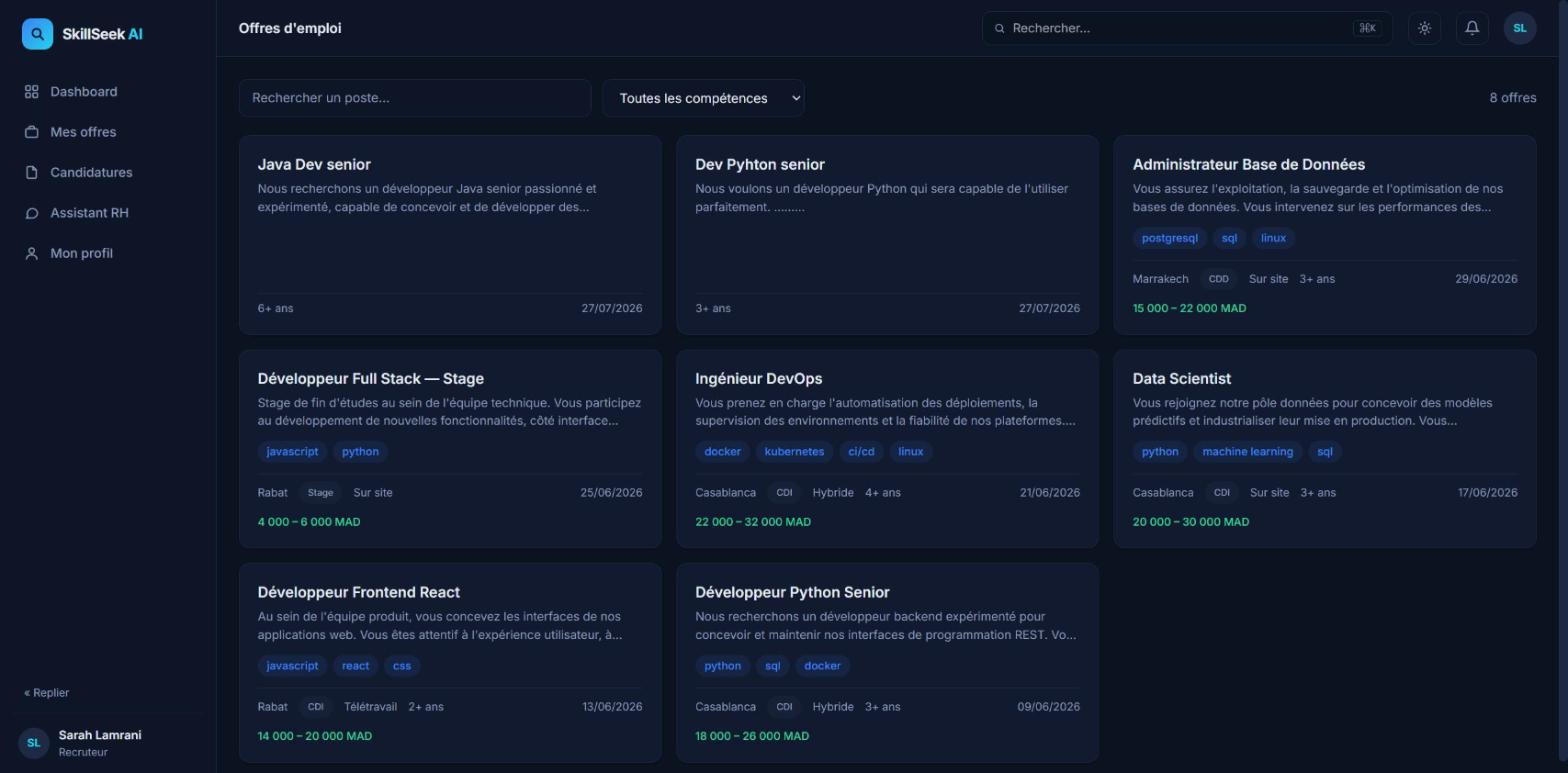
\includegraphics[width=0.86\textwidth]{captures/10_offres_publiees.jpg}
  \caption{Offres publiées, avec recherche et filtre par compétence.}
  \label{fig:c10}
\end{figure}

\begin{figure}[H]
  \centering
  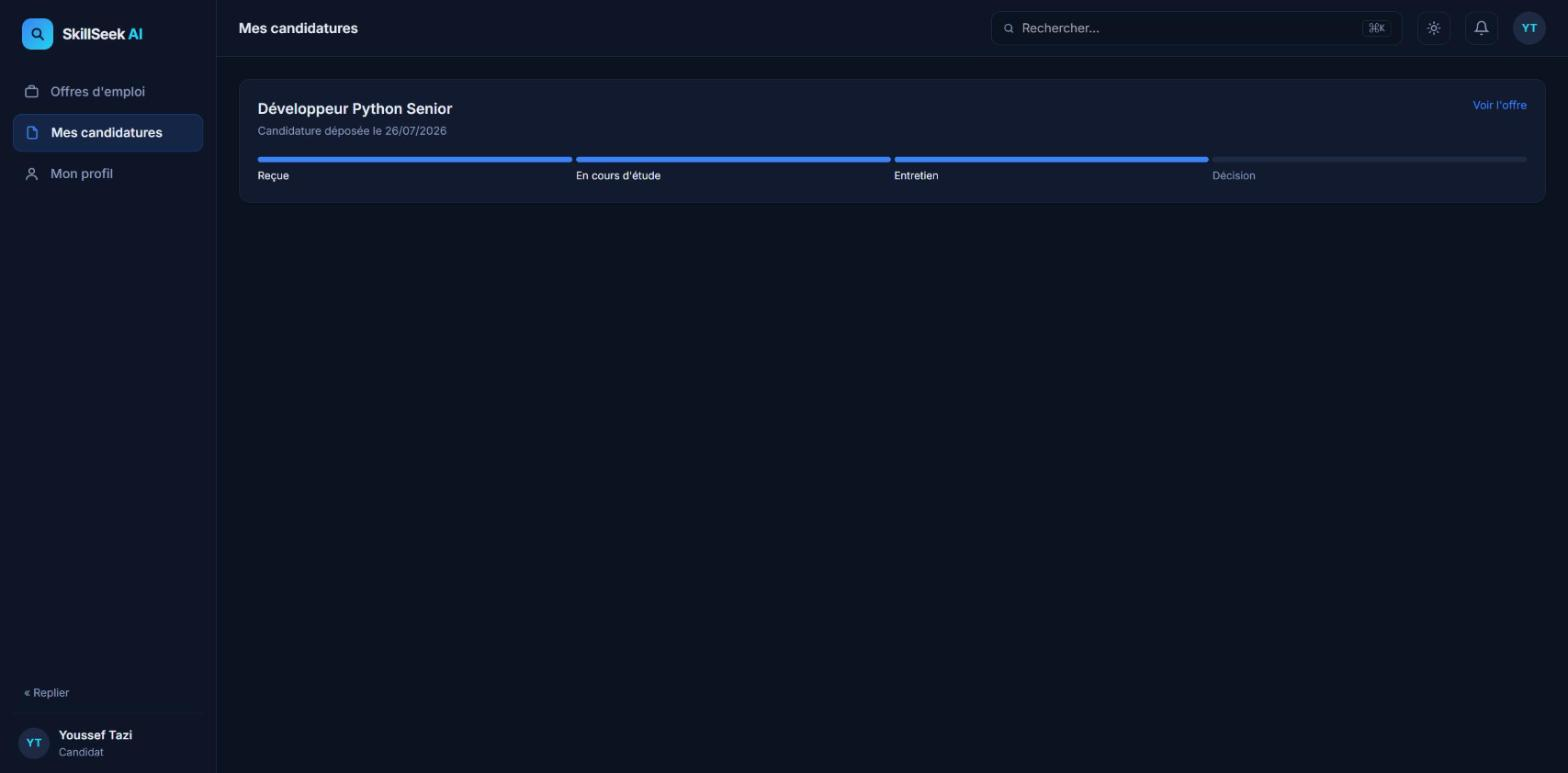
\includegraphics[width=0.86\textwidth]{captures/02_candidat_suivi_candidatures.jpg}
  \caption{Suivi des candidatures déposées. Aucune note n'est communiquée au
           candidat : seules les compétences manquantes le sont, car ce sont
           les seules qu'il puisse corriger.}
  \label{fig:c02}
\end{figure}

\subsection{Parcours du recruteur}

\begin{figure}[H]
  \centering
  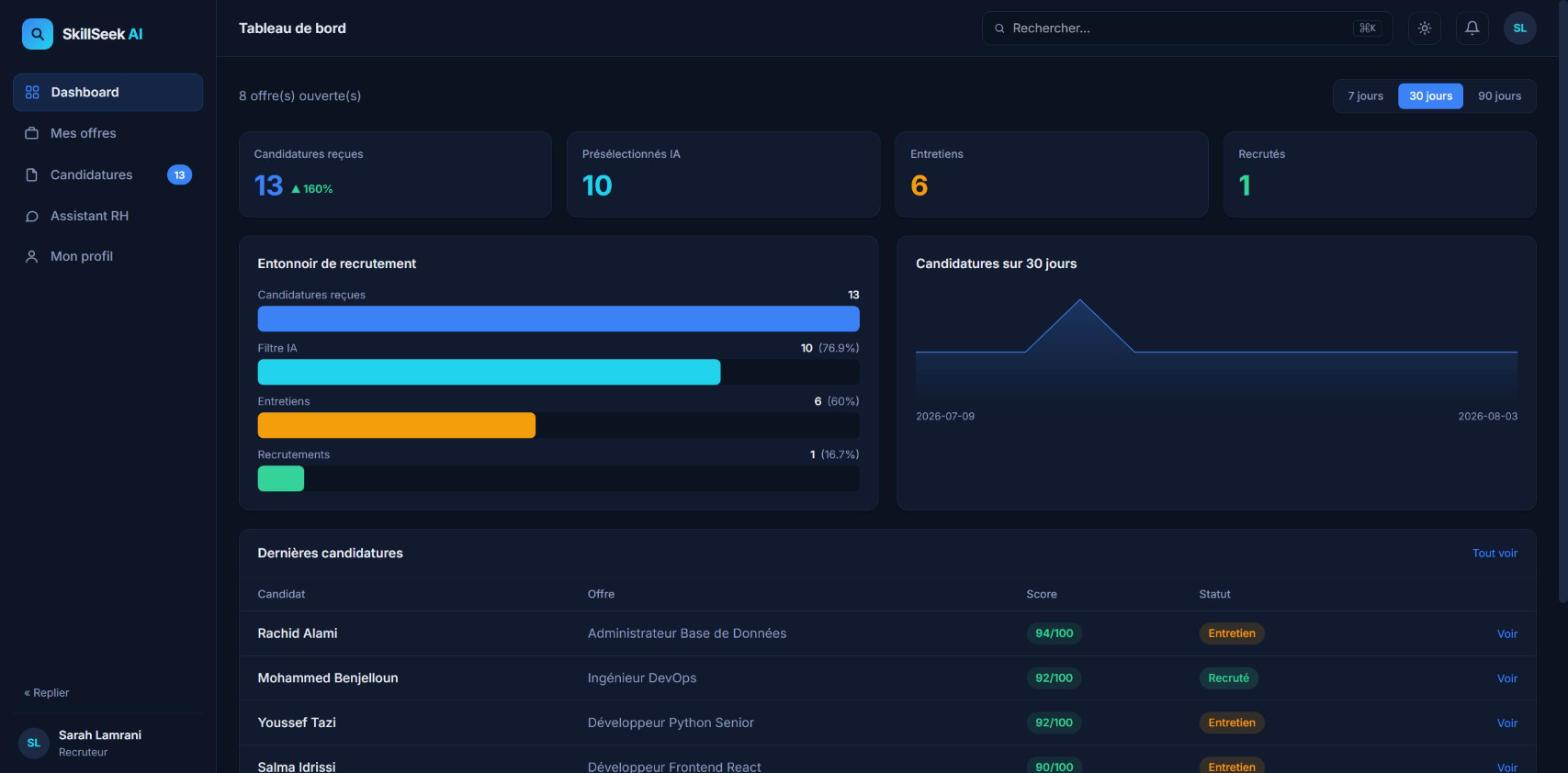
\includegraphics[width=0.86\textwidth]{captures/03_recruteur_tableau_de_bord.jpg}
  \caption{Tableau de bord du recruteur.}
  \label{fig:c03}
\end{figure}

\begin{figure}[H]
  \centering
  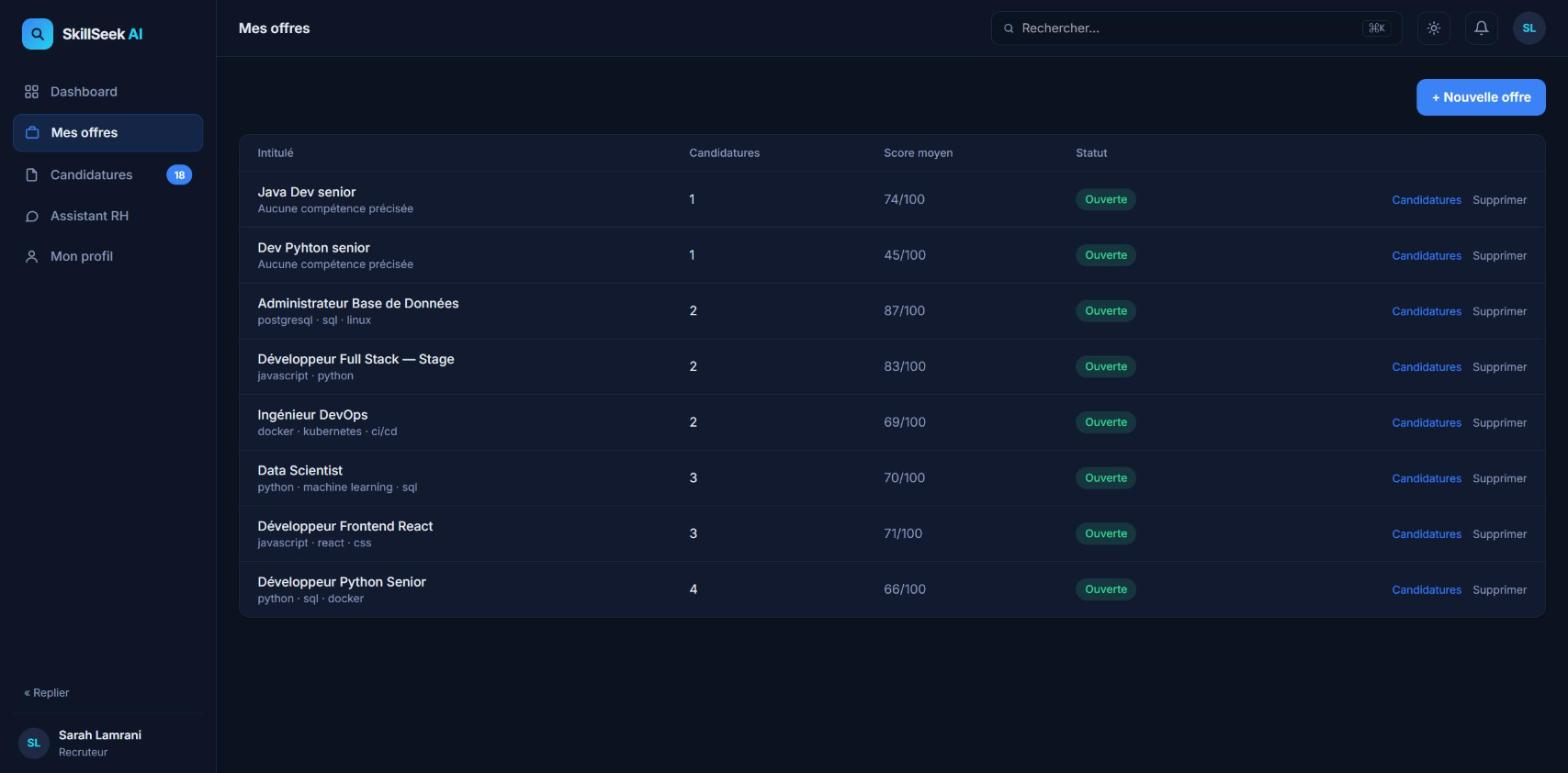
\includegraphics[width=0.86\textwidth]{captures/09_recruteur_mes_offres.jpg}
  \caption{Gestion des offres publiées par le recruteur.}
  \label{fig:c09}
\end{figure}

\begin{figure}[H]
  \centering
  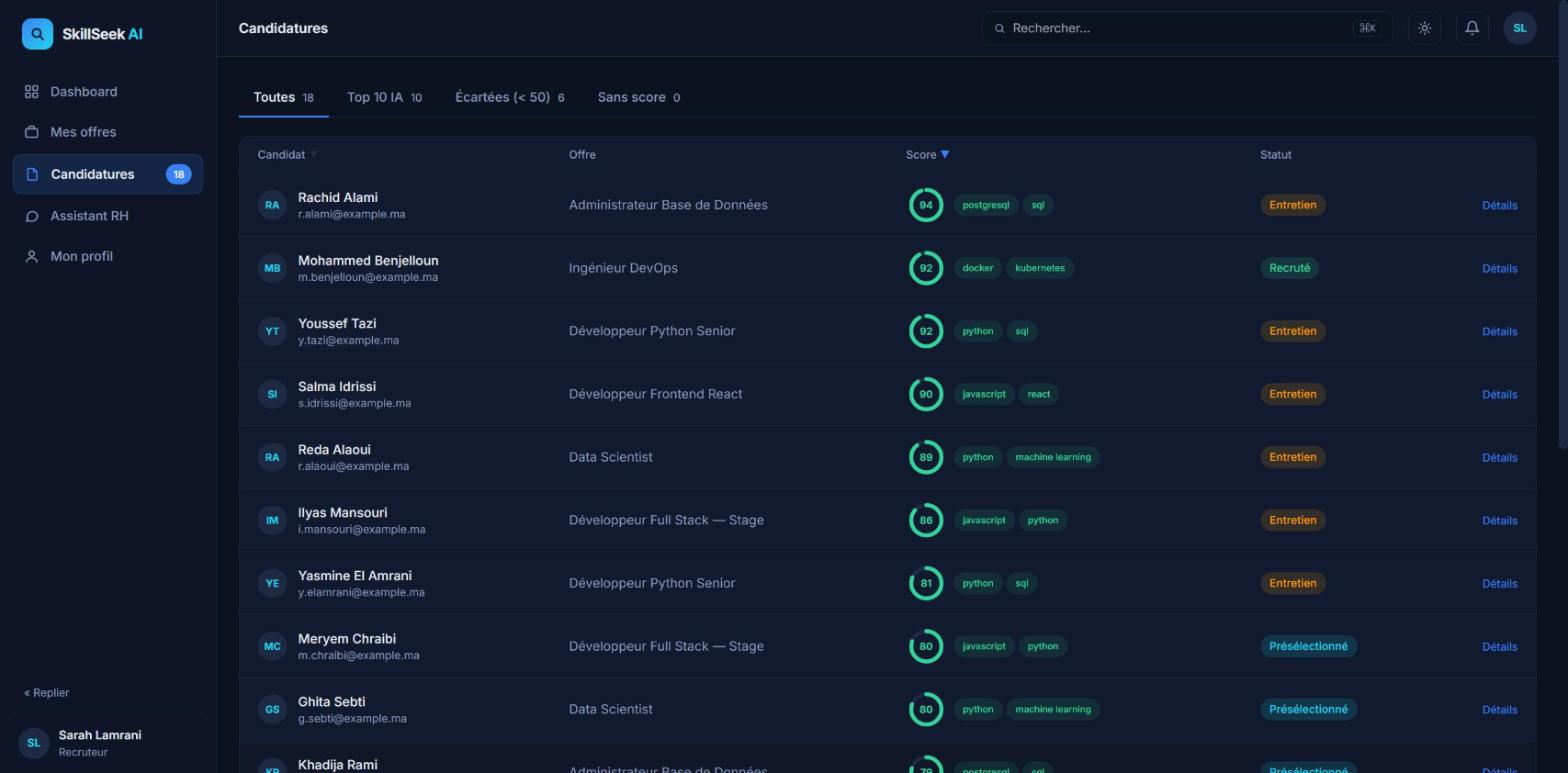
\includegraphics[width=0.86\textwidth]{captures/04_recruteur_candidatures_classees.jpg}
  \caption{Candidatures classées pour une offre, selon la règle RG-01.}
  \label{fig:c04}
\end{figure}

\begin{figure}[H]
  \centering
  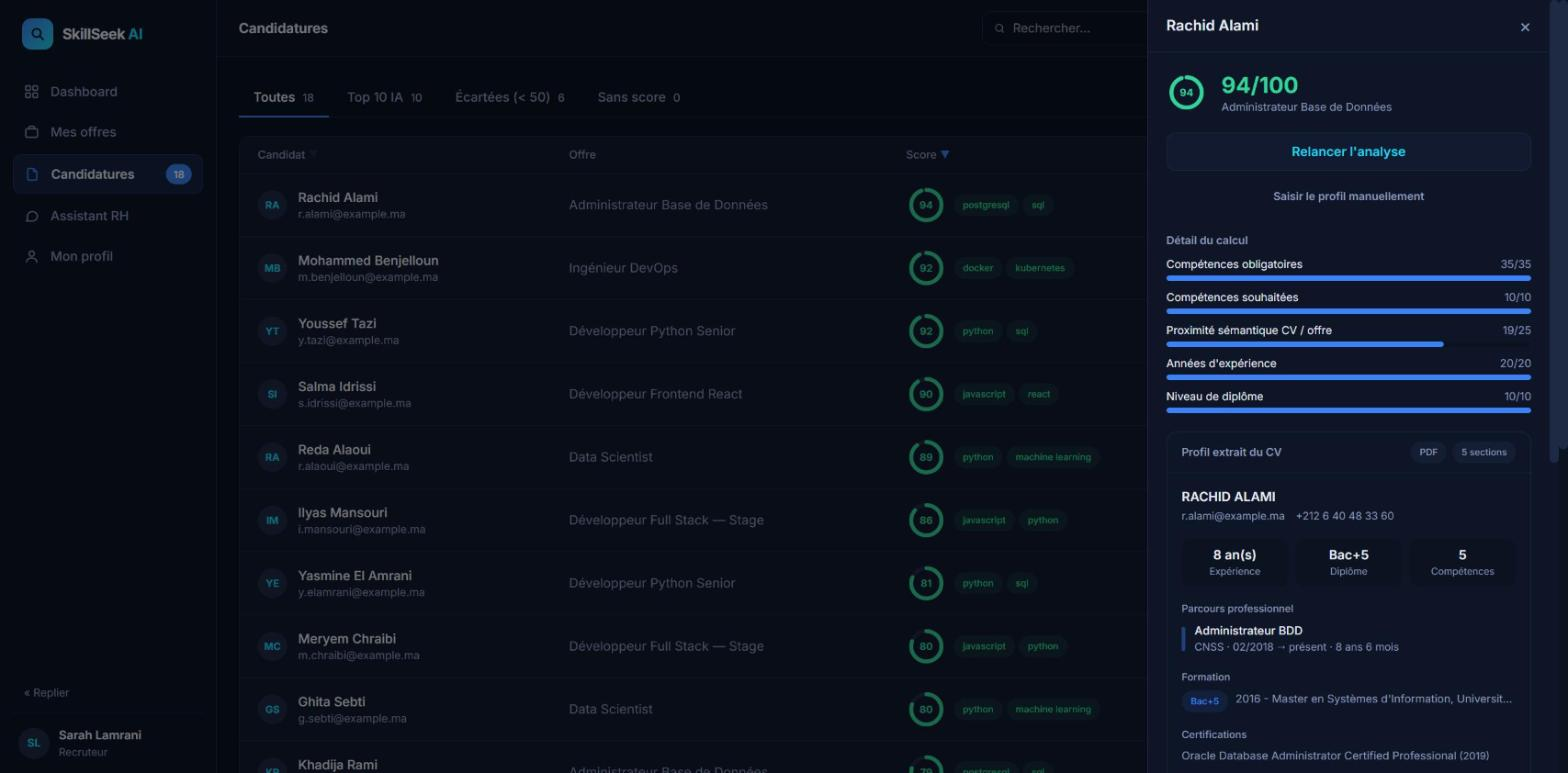
\includegraphics[width=0.86\textwidth]{captures/05_detail_score_profil_ats.jpg}
  \caption{Détail d'une note et profil reconstitué à partir du curriculum
           vit\ae{} : c'est l'écran qui porte la promesse d'explicabilité.}
  \label{fig:c05}
\end{figure}

\begin{figure}[H]
  \centering
  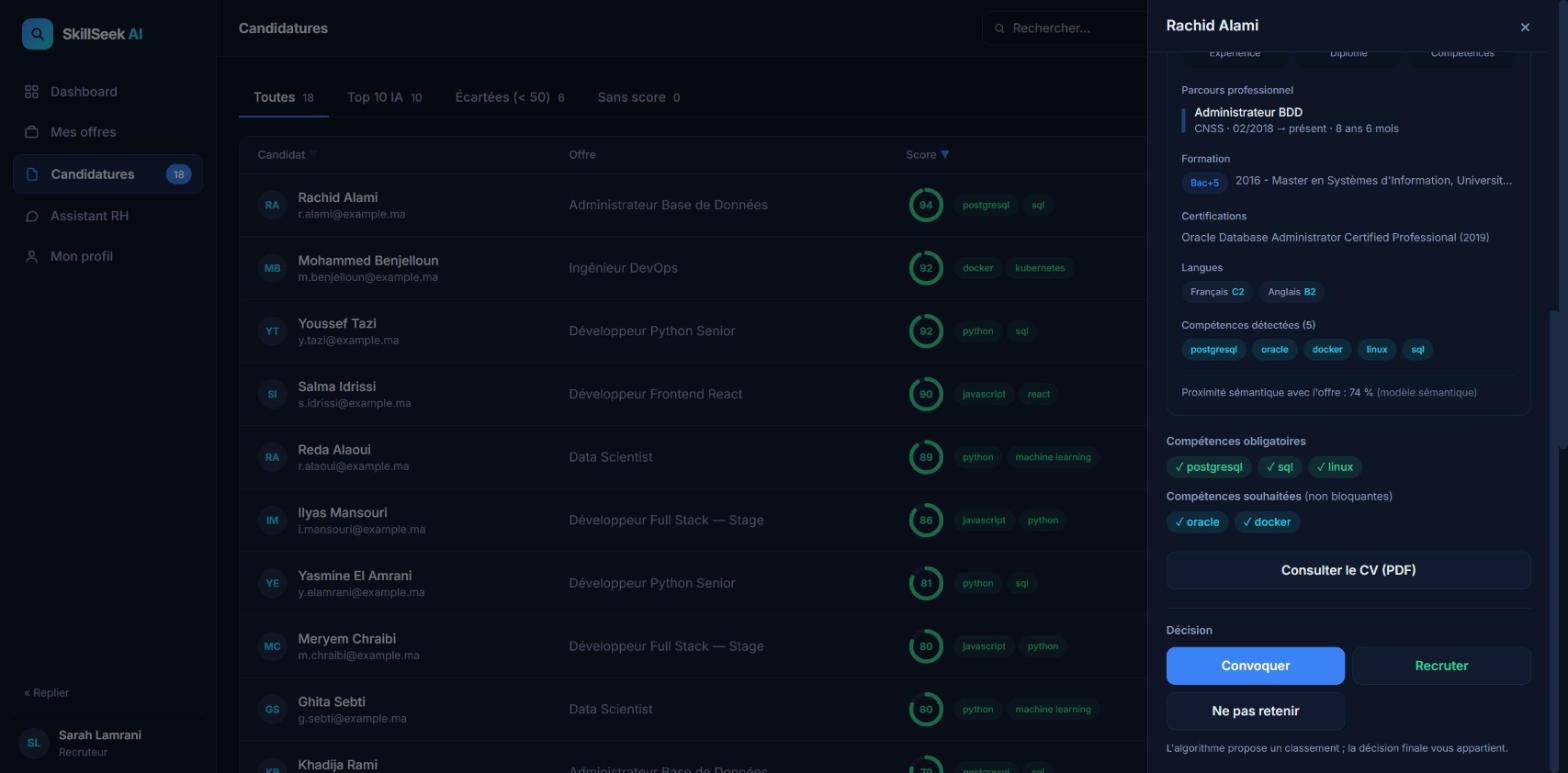
\includegraphics[width=0.86\textwidth]{captures/06_detail_score_bas_competences.jpg}
  \caption{Décomposition d'une note basse : la composante déficitaire est
           nommée.}
  \label{fig:c06}
\end{figure}

\begin{figure}[H]
  \centering
  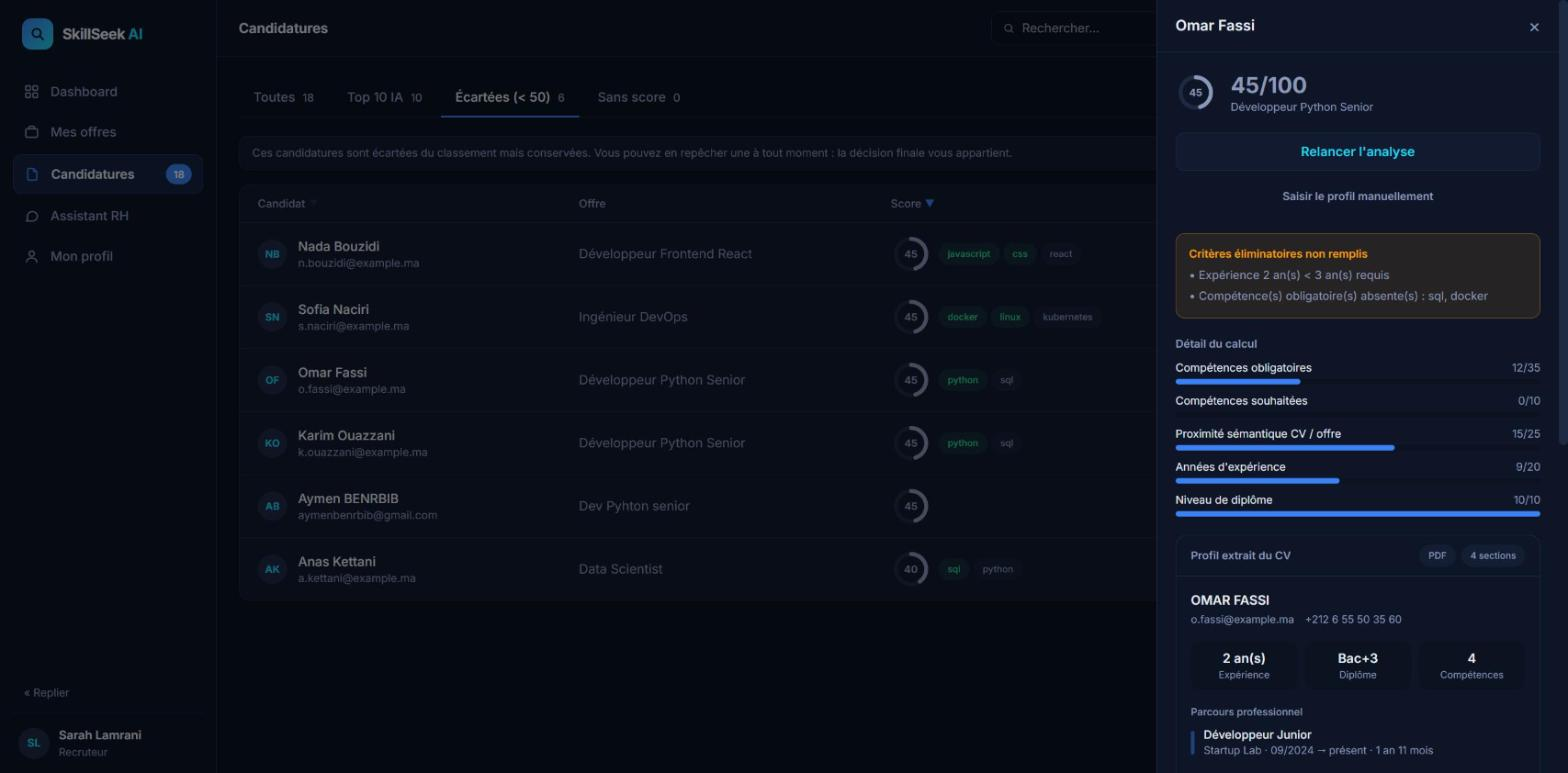
\includegraphics[width=0.86\textwidth]{captures/07_candidature_ecartee_motifs.jpg}
  \caption{Candidature écartée du classement : le motif est affiché, et la
           candidature demeure consultable et repêchable.}
  \label{fig:c07}
\end{figure}

\begin{figure}[H]
  \centering
  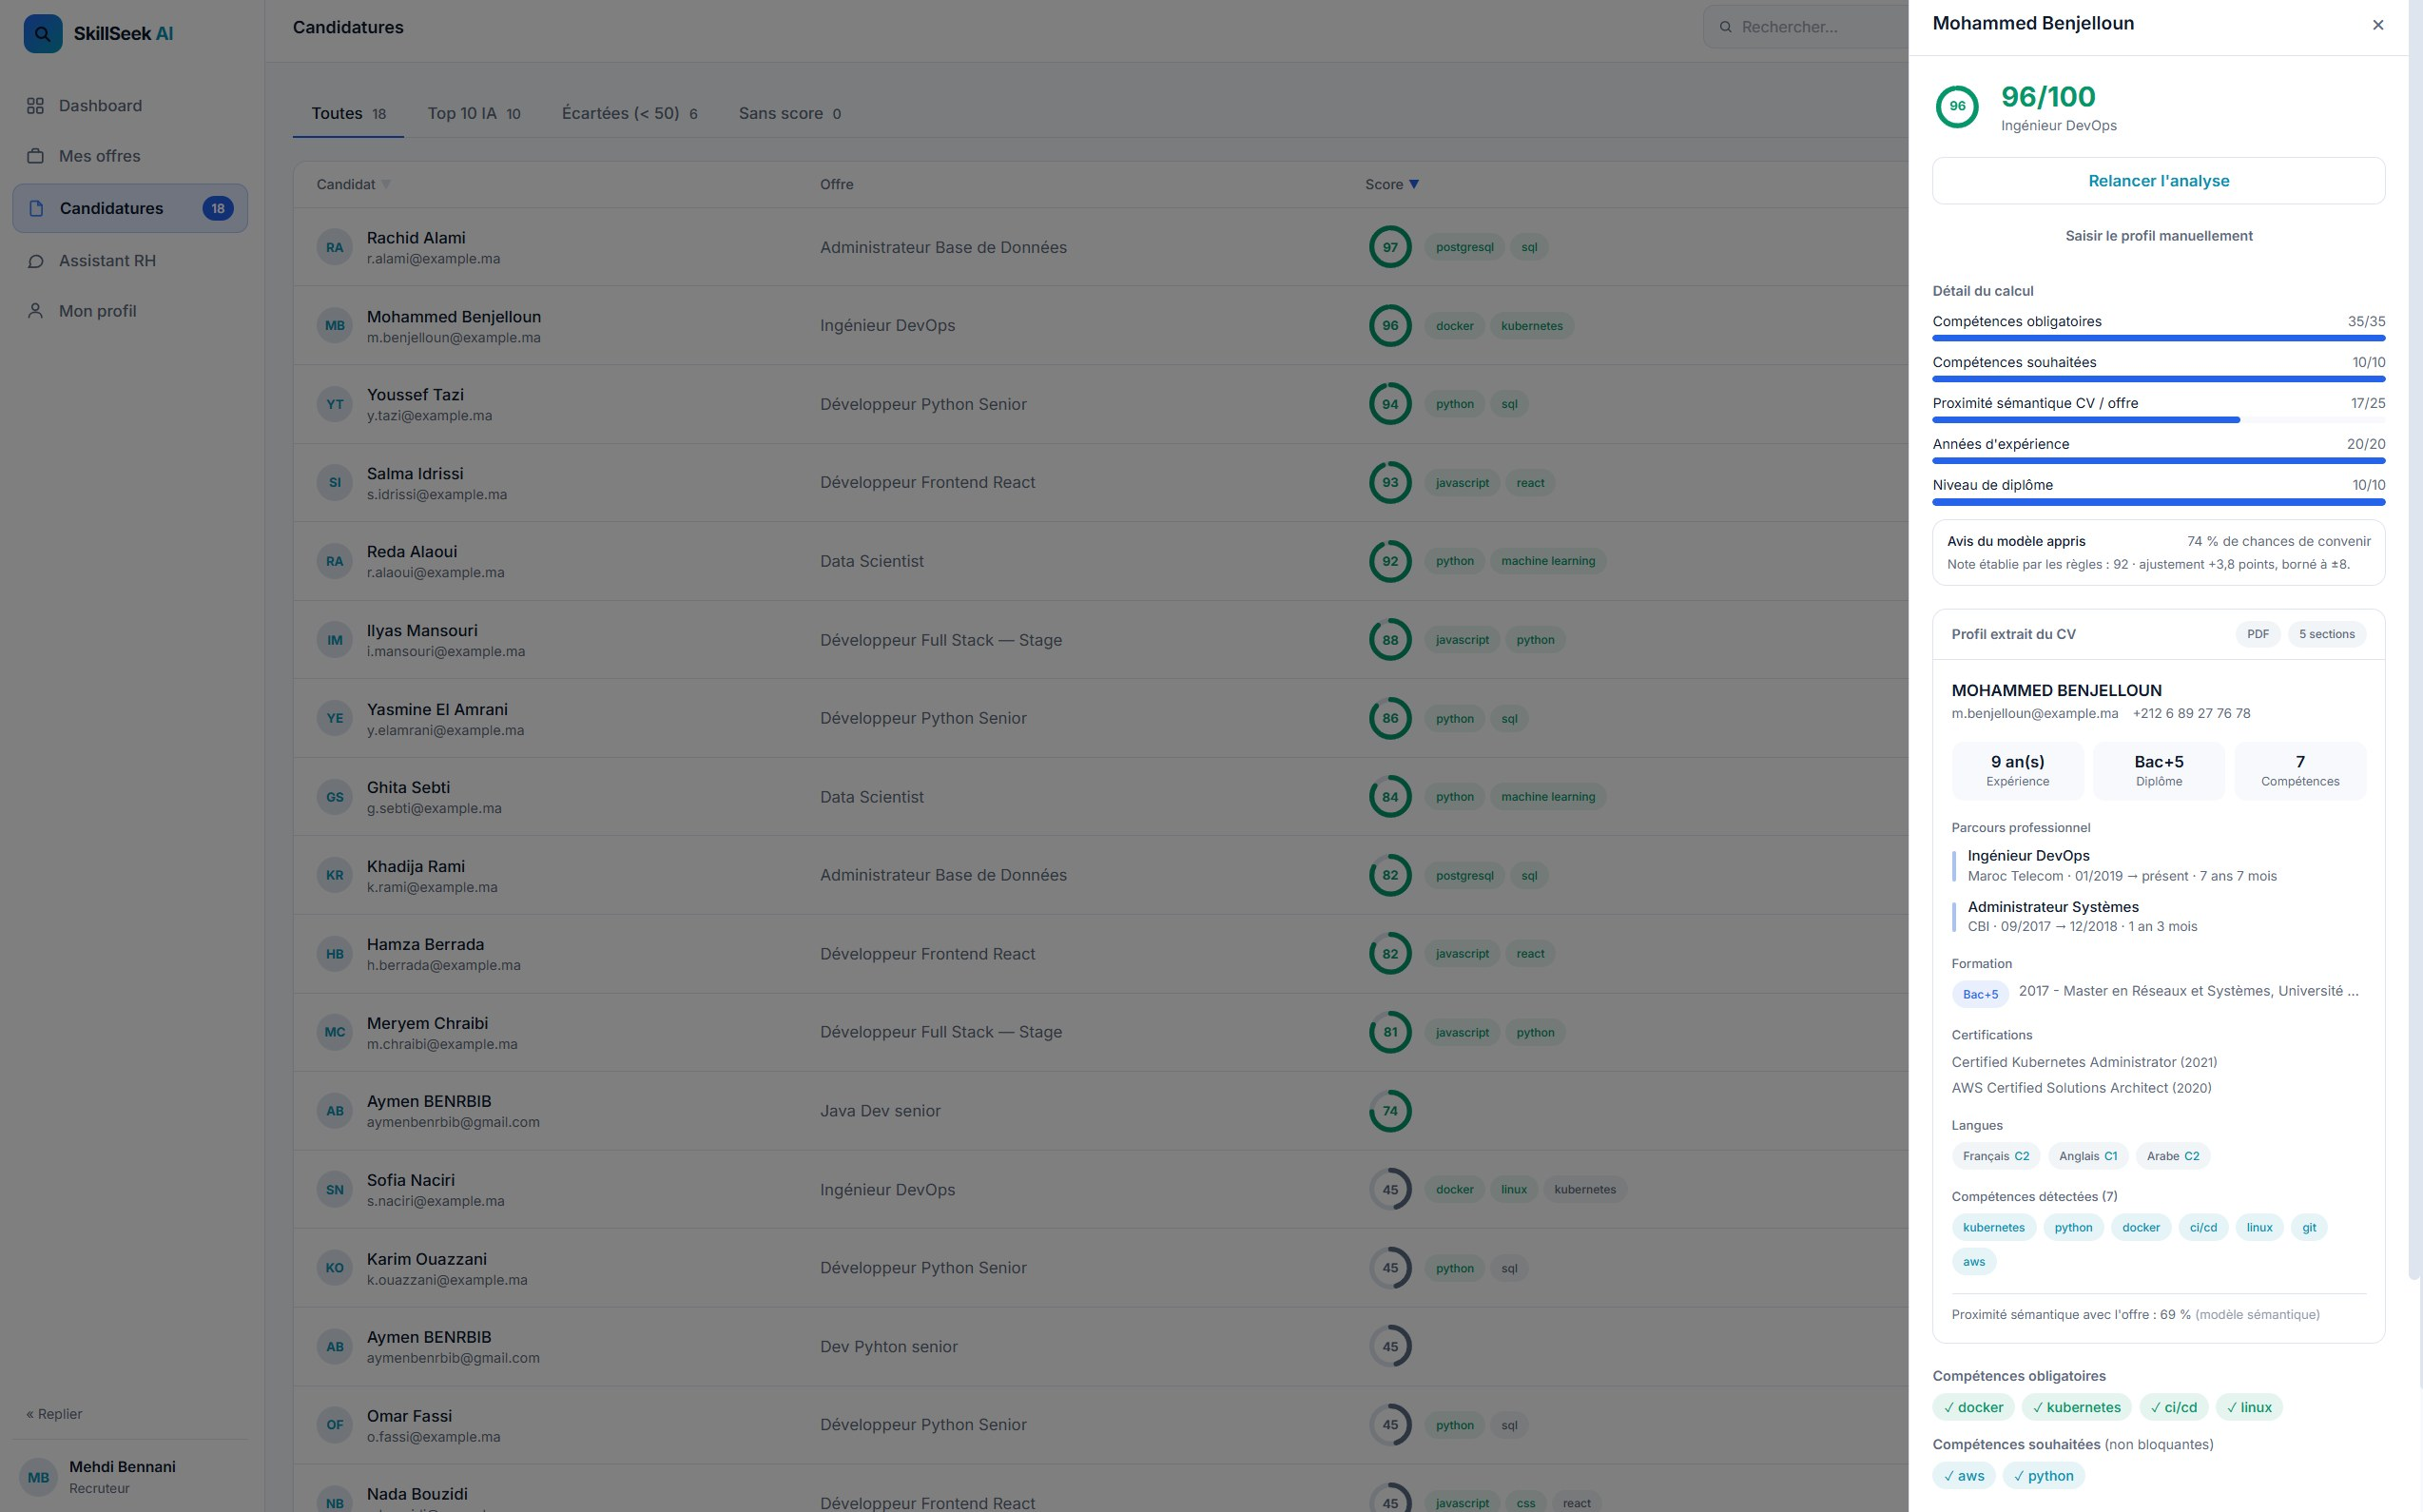
\includegraphics[width=0.86\textwidth]{captures/15_avis_modele.jpg}
  \caption{Avis du modèle appris, présenté séparément de la note fondée sur
           les règles, et borné à huit points.}
  \label{fig:c15}
\end{figure}

\begin{figure}[H]
  \centering
  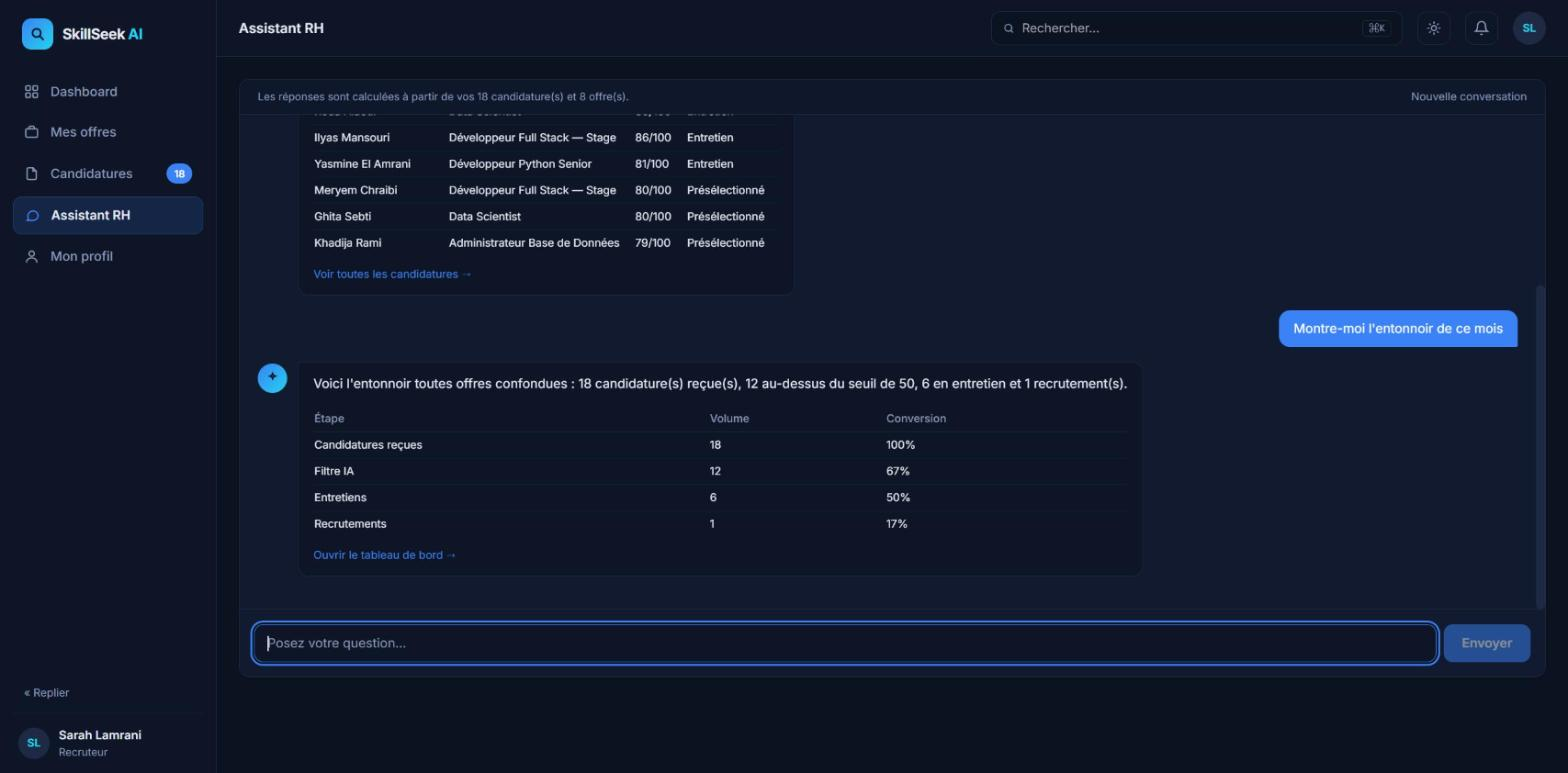
\includegraphics[width=0.86\textwidth]{captures/08_assistant_rh_entonnoir.jpg}
  \caption{Assistant de recherche documentaire, restreint au périmètre de
           l'utilisateur.}
  \label{fig:c08}
\end{figure}

\subsection{Parcours de l'administrateur}

\begin{figure}[H]
  \centering
  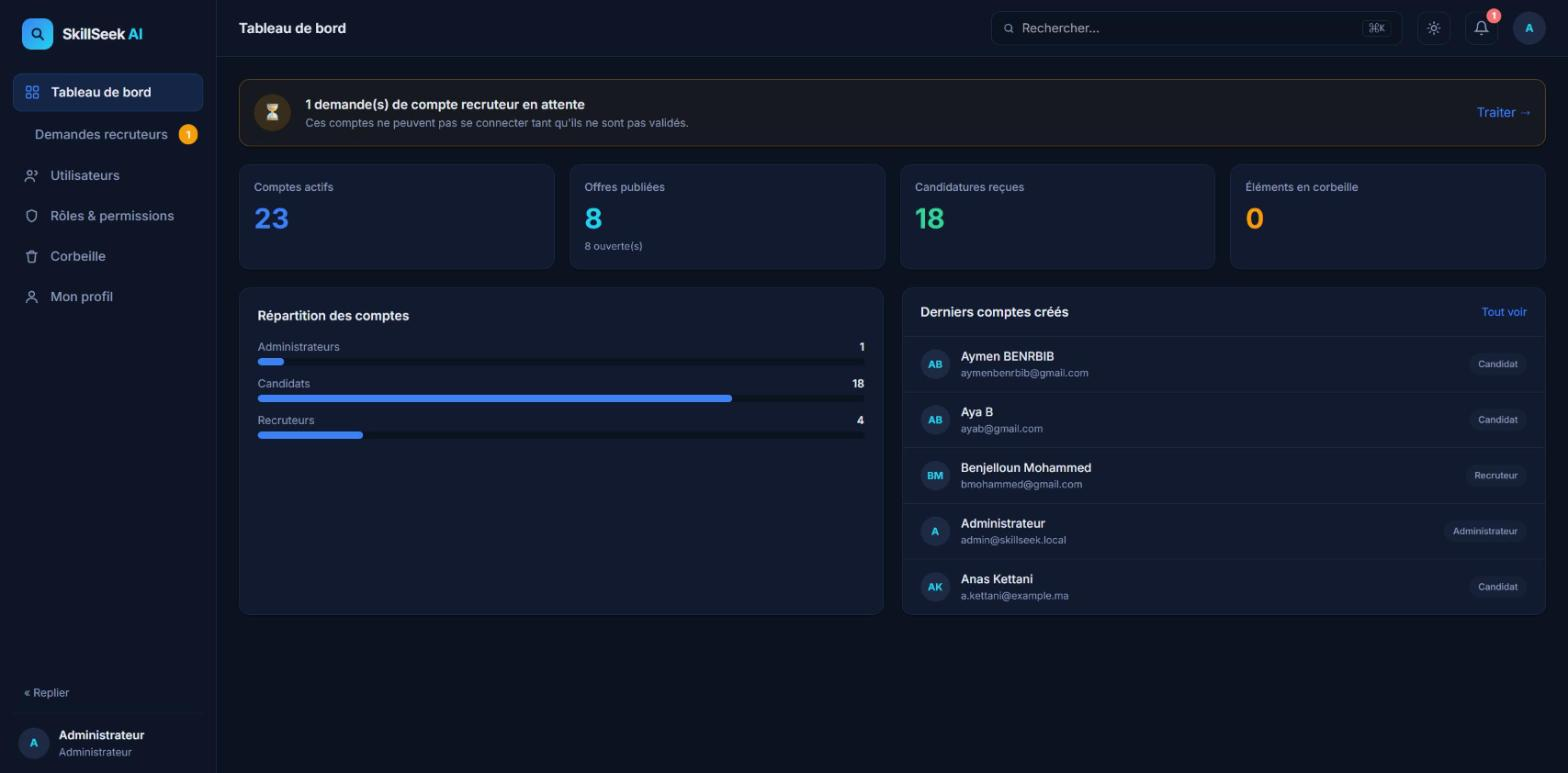
\includegraphics[width=0.86\textwidth]{captures/11_admin_tableau_de_bord.jpg}
  \caption{Tableau de bord de l'administration.}
  \label{fig:c11}
\end{figure}

\begin{figure}[H]
  \centering
  
\includegraphics[width=0.86\textwidth]{captures/12_admin_validation_recruteurs.jpg}
  \caption{Validation des comptes recruteurs : publier une offre au nom de
           l'entreprise engage celle-ci, d'où cette étape.}
  \label{fig:c12}
\end{figure}

\begin{figure}[H]
  \centering
  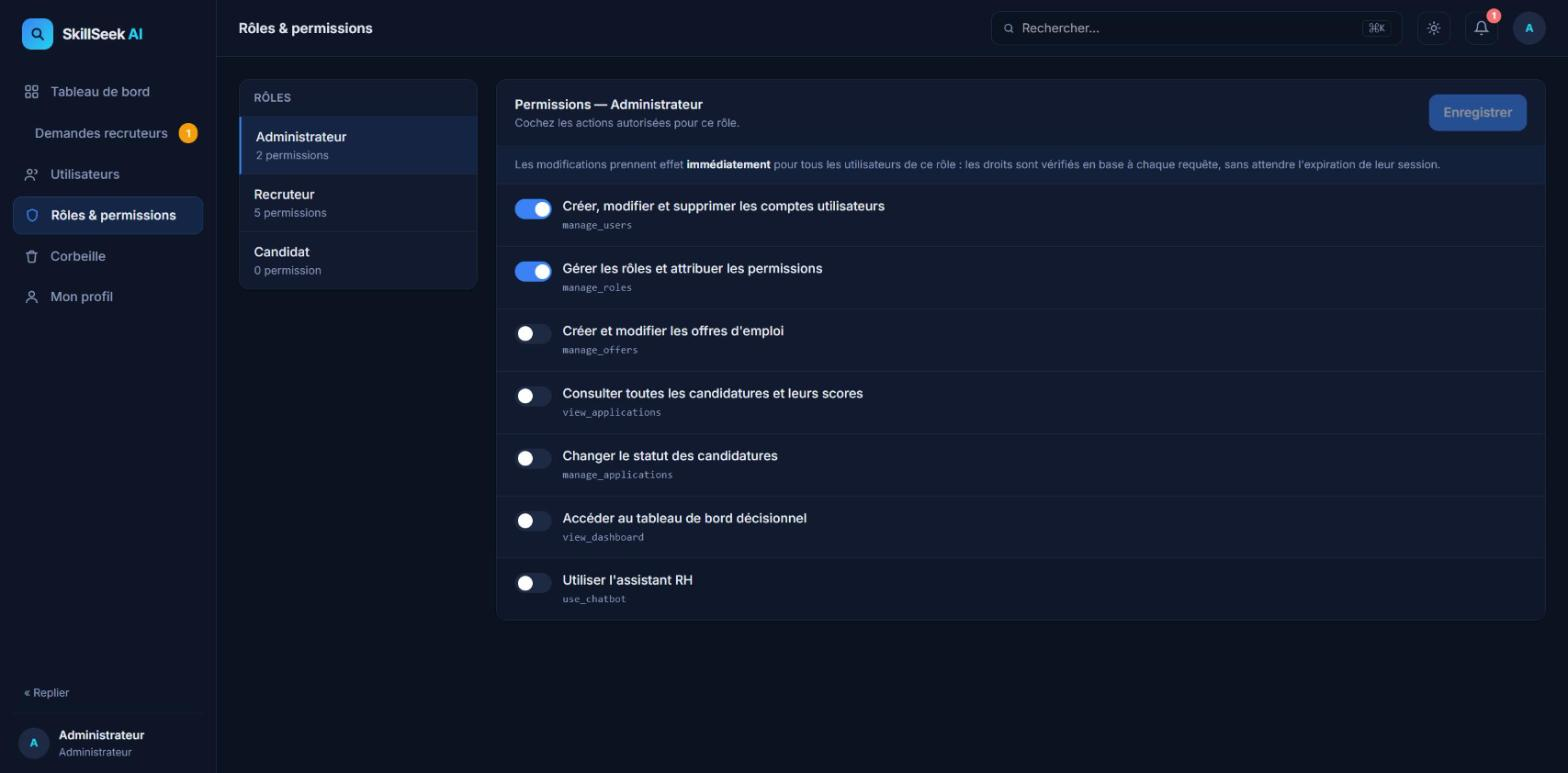
\includegraphics[width=0.86\textwidth]{captures/13_admin_roles_permissions.jpg}
  \caption{Matrice des rôles et des permissions. Un retrait de droit prend
           effet immédiatement (règle RG-02).}
  \label{fig:c13}
\end{figure}

\begin{figure}[H]
  \centering
  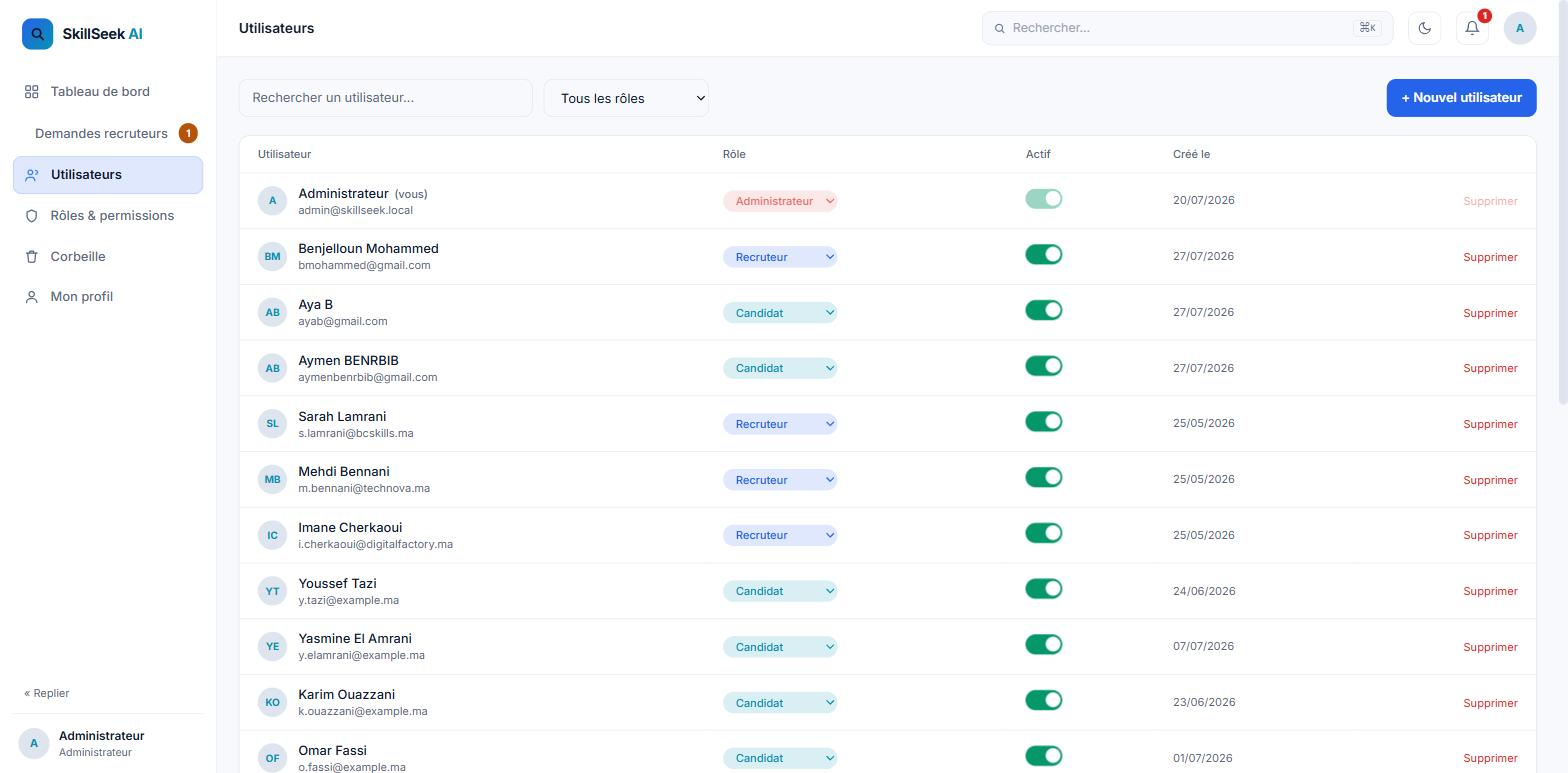
\includegraphics[width=0.86\textwidth]{captures/14_mode_clair_utilisateurs.jpg}
  \caption{Gestion des comptes utilisateurs, en thème clair.}
  \label{fig:c14}
\end{figure}

\subsection{Chaîne d'intégration}

\IfFileExists{captures/ci_1_executions.jpg}{%
\begin{figure}[H]
  \centering
  \includegraphics[width=0.86\textwidth]{captures/ci_1_executions.jpg}
  \caption{Historique des exécutions de la chaîne d'intégration : chaque
           poussée déclenche les sept travaux.}
  \label{fig:ci1}
\end{figure}}{}

\IfFileExists{captures/ci_2_graphe_travaux.jpg}{%
\begin{figure}[H]
  \centering
  \includegraphics[width=0.86\textwidth]{captures/ci_2_graphe_travaux.jpg}
  \caption{Graphe d'une exécution : les travaux parallèles, leurs
           dépendances et leurs durées respectives.}
  \label{fig:ci2}
\end{figure}}{}

\IfFileExists{captures/ci_3_qualite.jpg}{%
\begin{figure}[H]
  \centering
  \includegraphics[width=0.86\textwidth]{captures/ci_3_qualite.jpg}
  \caption{Tableau de bord de l'analyse de qualité : sécurité, fiabilité et
           maintenabilité.}
  \label{fig:ci3}
\end{figure}}{}

\subsection{Chaîne de livraison}

\begin{figure}[H]
  \centering
  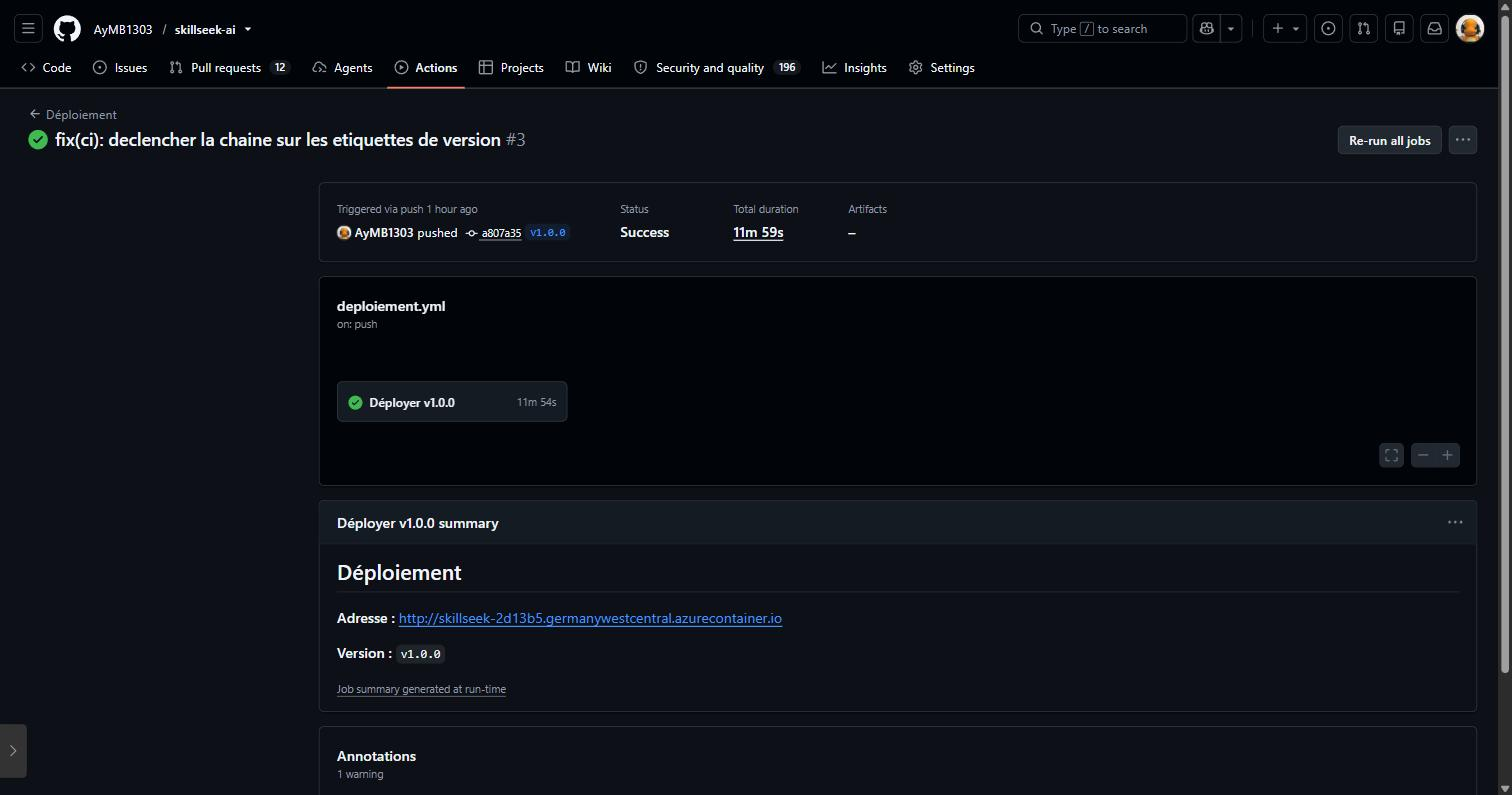
\includegraphics[width=0.86\textwidth]{captures/cd_1_resume_v1.0.0.jpg}
  \caption{Déploiement déclenché par la pose de l'étiquette de version.}
  \label{fig:cd1}
\end{figure}

\begin{figure}[H]
  \centering
  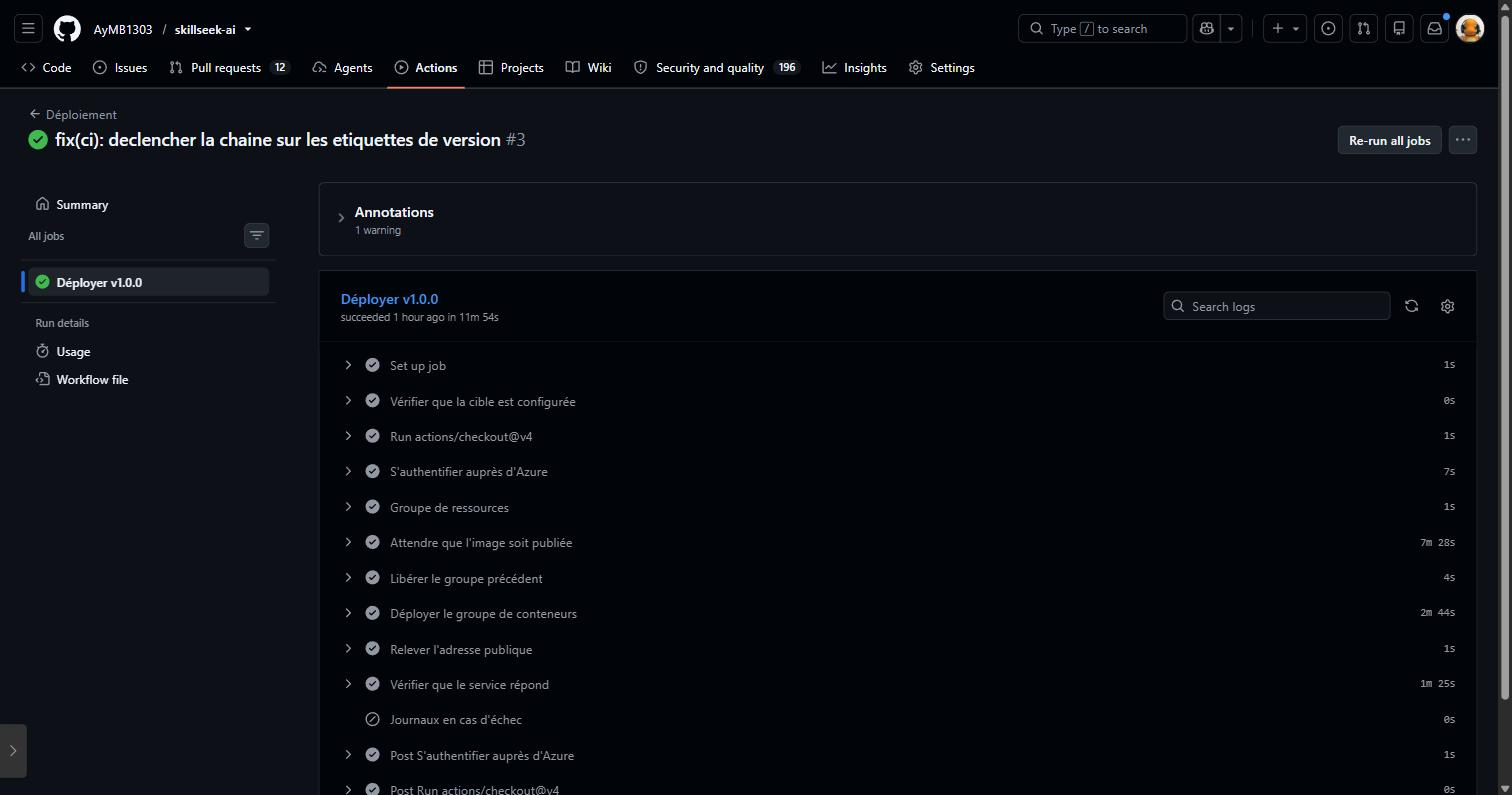
\includegraphics[width=0.86\textwidth]{captures/cd_2_etapes_workflow.jpg}
  \caption{Étapes du déploiement : attente de l'image au registre, création
           du groupe de conteneurs, puis interrogation de la sonde depuis
           l'extérieur.}
  \label{fig:cd2}
\end{figure}

\end{document}
